\documentclass[10pt,journal,final,]{article}
\usepackage{amsmath}
\usepackage{makeidx}
\usepackage{cite}
\usepackage{listings}
\usepackage{bm}
\usepackage{amssymb}
\usepackage{amsthm}
\usepackage{stmaryrd}
\usepackage{algorithm}
\usepackage{algorithmic}
\usepackage{verbatim}
\usepackage{graphicx}
\pagestyle{plain}

% If you don't want to indent each first paragraph after sectional headings, comment this
\usepackage{indentfirst}

\newcommand{\emptyline}{\vspace{\baselineskip}}
\newcommand{\llb}{\llbracket}
\newcommand{\rrb}{\rrbracket}

\lstset{
  language=C,
  basicstyle=\footnotesize\ttfamily,
  otherkeywords={*,then,:=,fi,goto,end}
}

\theoremstyle{definition}
\newtheorem{definition}{Definition}[section]
\newtheorem{theorem}{Theorem}[section]

\begin{document}

\title{Program Repair Based on SMT}
\author{Zhang Ling, Wan Hai, Peng Yi, Guo BoTing}
\date{\today}
\maketitle

\begin{frontmatter}
\begin{abstract}
\label{section:Abstract}
% 类似C语言等拥有控制语句的高级语言,在自动修复的过程中推理其复杂的数据依赖和控制关系往往是比较困难的。
For high-level programming language like $C$, it is hard to deduce its complicated data dependency and control flow during the progress of automatic repair.
% 通过将C语言程序转换为布尔程序,本文得以完整模拟布尔程序,收集所有使程序出错的错误路径并推导出正确的布尔修复,并最终转换为修复后的C语言程序,使得整个C语言程序的修复过程完全自动化。
By converting $C$ program to boolean program and simulating its execution, we managed to collect all bad paths that lead the program into error states, and deduce the exact boolean repair statement by excluding all the bad routes. The repaired boolean program can be converted back to $C$ program, thus the whole procedure of repairing can be deemed fully automatic.
% 文末,我们给出了根据这些方法实现的C语言程序修复工具的相关设计,并采用了TCAS测试集来验证工具的正确性及有效性。
We further give out the design and architecture of the automatic repairing tool that is implemented based on this method, and put it under testing to verify its effectiveness and correctness.
\end{abstract}
\begin{keyword}
% 关键词:代码修复、布尔程序、逆向转换
Code Repair, Boolean Program, SMT, Reverse Conversion
\end{keyword}
\end{frontmatter}
\section{Introduction}
\label{section:Introduction}
\subsection{Background}
\label{section:Background}
% 调试是发现和减少计算机程序或电子硬件中的错误或缺陷的有序过程,使其按照预期的行为执行。
Debugging is the process of finding and resolving bugs or defects that prevent correct operation of computer software or a system\cite{APD}.
% 程序调试的过程包括错误定位和代码修复两个阶段。
The process of debugging requires {\it fault localization} and {\it program repair}\cite{SPBPRUS}.
% 错误定位指发现并且确定代码错误的所在位置
Fault localization means finding the location of faults,
% 代码修复则是对已定位的错误语句进行一系列的操作来进行错误修复,主要是通过构建正确的语句并移除错误的语句来进行错误修复。
while program repair means fixing the faults, mostly done by developing correct statements and removing faulty ones\cite{LCoPF}.
% 代码错误的修复大多数时候需要人工进行,比较困难和耗费时间
For most cases, such procedure has to be done manually, which can be notoriously hard and time consuming.

% 在软件系统的维护过程中,软件修复是其中的首要任务,在维护过程中发现问题往往需要通过人工去跟踪定位分析,经过再次的开发和测试之后才能发布软件系统的补丁,修复系统错误。
Program repair takes up the most parts of software maintenance. Finding a bug requires manual tracking and analysis, and only after further development and testing can the update patch be published to fix the bug\cite{SCaMC}.
% 这种维护技术存在的最大问题就是软件修复占用的周期相对较长,并且在软件修复的工程中只能停止当前软件服务或者暴露软件本身的缺陷来继续执行,这样对软件的可用性和安全性都可能造成严重影响,并且在软件修复周期内造成巨大花费
Fixing a bug in such maintenance fashion takes up too much time, while the company can only choose to terminate the software or keep it running at the risk of exposing its defect, which could bring great threat to the software's availability and security. Both choices can bring great financial cost to the company\cite{CMfFSLCP}.
% 在已知的一些报告中也指出,软件的维护,通常指软件系统发布之后对其的改动,造成的花费可能达到整个软件项目的90%。
Some reports place software maintenance, traditionally defined as any modification made on a system after its delivery, at 90\% of the total cost of a typical software project\cite{CMfFSLCP}.
% 这些花费主要用在修改更新现有的代码、修复系统的缺陷以及其他涉及到该系统的软件。
Modifying existing code, repairing defects, and otherwise evolving software are major parts of those costs\cite{AiSE}.
% 然而,在软件系统中,存在缺陷的数量远远超过了可以用来解决这些缺陷的资源
However, the number of outstanding software defects typically exceeds the resources available to address them.
% 即使在一个成熟的软件项目里,由于缺少开发资源来解决每一个发现的缺陷,系统被迫伴随着已知或未知的各种错误一起发布
Even a mature software projects would be forced to ship with both known and unknown bugs, because they lack the development resources to deal with every defect. For example, in 2005, one Mozilla developer claimed that, “everyday, almost 300 bugs appear, far too much for only the Mozilla programmers to handle.”

% 发现存在问题后的一系列修复过程都靠人工完成是修复周期长和花费巨大的一个重要原因,这样导致修复的时效性较差。
The great cost of program repair comes from the necessity of manual intervene\cite{SFTiaCA:TaRM}.
% 针对此问题,软件自动化和智能化修复的研究便成为一个热点。
To solve such problem, research on automatic software repairing has been in the spotlight.
% 自动化调试技术能够明显地减少调试的花销。
% Automation of fixing software bugs can greatly reduce the cost penalties of debugging\cite{OtAoFSB}.
% 在自动化调试方面,传统的研究集中于对错误定位的研究,大多数的代码修复仍然是通过手工完成的。
% As for automatic debugging, traditional research focuses on fault localization, while program repair is still mostly done by human.
Unfortunately, most traditional research focuses on automatic fault localization, while program repair is still done by human.
% 目前已提出的一些代码修复方法令我们能够相对容易地发现代码出现缺陷的原因,但是他们的精度依然不足以给出单独的具体的代码修复建议,开发人员仍然需要去设计及开发补丁。
Many effective methods of program repair have been proposed in the recent years, which do make it easier to locate the cause of software defects, but they are still not accurate enough to come up with a concrete advice for program repair: the job of designing and developing update patch still needs to be done by human developers.
% 开发人员需要的是使系统能够从错误中恢复并且使得这些错误不会再发生。针对这种情况采取的是有计划的修复,也就是说,对于能够预知的错误类型有着定义好的修复策略。
What developers need is to recover the software system from failure and make sure such error will not happen again\cite{MBAfSHS}. In this circumstance, premeditated repair is generally applied, meaning pre-defined repairing strategies for predicted errors.

% 已经提出的代码修复方法大多都是基于原始的程序来通过形式化规范或者测试用例进行恢复的,而像C语言一样具有控制流结构的程序很难直接对其复杂的数据和控制关系进行推理
The program repairing methods proposed in recent years are mostly based on formal specifications or test cases, but it is hard to deduce the complicated data dependencies and control flows for high-level programming language like $C$.
% 在针对程序的控制流结构进行修复的时候,需要用更简单易推理的语言或者规范
Thus, we need a different language or specification which is easy to deduce its control flow structure as we try to repair the program automatically.
% 2000年,微软的研究人员提出了一种新的软件分析模型和过程语言——布尔程序
In 2000, a new model and process for program analysis was proposed by Microsoft researchers -- the boolean program\cite{BP:aMaPfSA}.
% 布尔程序是跟C语言一样有常规的控制流结构的命令式语言:有函数、递归,同样有全局变量和局部变量。
Boolean program is similar to C program: they both have functions and recursions, global and local variables\cite{Bb:aSMCfBP}.
% 唯一的区别就是所有的变量都是布尔类型。
The difference is that all variables in boolean program are of boolean type and no additional storage is available.
% 布尔程序同时还支持断言,并行赋值和非确定性
Boolean programs also support assertions, parallel assignments, and nondeterminism.

% 布尔程序在某种程度上可看作是接受上下文无关语言的下推自动机,它的可达性问题和终止性都是可确定的
To some extent, boolean program can be considered as a push-down automaton which accepts context-free language, its reachability and termination are both decidable\cite{CFLaPDA}.
% 布尔程序可看作是C程序的一个抽象表示,因为布尔变量能够代表C程序下的任意谓词,布尔程序能明确地捕捉到数据和控制之间的相关性
Boolean programs can be thought of as an abstract representation of C programs as it explicitly captures the correlations between data and control flow, in which boolean variables can represent arbitrary predicates over the unbounded state of a C program.\cite{APAoCP}.
% 布尔程序的这些特性使得它在利用数据和控制关系进行推理的时候非常有用。
Such characteristics of boolean program make it a suitable tool for data and control flow deduction.
% 过去针对代码修复的研究中有学者利用了布尔程序的这些特性,从实验结果来看,这种基于控制流结构来进行代码修复的方法非常有效
Boolean program has already been applied in several program repair research\cite{RoBPwaAtC}, and judged by the experimental results, repairing program based on its control flow structure is effective.
% 然而,该方法并没有做到完全的自动化,在针对布尔程序得到修复之后,仍然需要通过人工的干预,需要根据得到的布尔修复人工地转换为C程序的修复,并且转换后满足规范的结果可能不是唯一的,同样需要人工去进行选择
However, such method is not fully automatic: after repairing the boolean program, the boolean repair statement still needs to be converted back to $C$ language by human, and the results that satisfy the specification after conversion might not be unique, it is still human's job to pick one among them.
% 程序员仍然需要花时间去得到C程序的补丁,这在某种程度上并未完全达到代码自动化修复的目的

% 基于布尔程序的特性,选其作为代码修复过程的中间语言来进行分析和修复是一个值得研究的方法。
Judging by the characteristics of boolean program, it will make a suitable intermediate language for program analysis and repair.
% 本文的工作便在利用布尔程序进行代码修复的基础上更进一步,在利用控制流结构对代码进行分析后找到布尔程序修复,并将该修复代码逆向转换为可读可执行的C语言代码,而无需人工进行布尔程序到C程序的转换
The work we present here goes one step beyond the former research: we analyze the program based on its control flow structure to find out the appropriate boolean repair, and convert the repair statement back to readable and executable $C$ statement automatically, totally without human intervene.
% 这样,对C程序的错误修复,可以变成从C程序转换成布尔程序、修复布尔程序、把修复布尔程序结果还原成C程序三个步骤,并且每个步骤都自动完成,从而完成修复的完全自动化的过程
The process of repairing a $C$ program can be considered as three steps: convert the $C$ program into boolean program, repair the boolean program and convert the repaired result back to $C$ program. Each step shall be done automatically to achieve fully automatic program repair.
% 本文着重研究了其中的第三步。
We focus on automatizing the third step.

\subsection{Research situation}
\label{section:ResearchSituation}
% 在代码自动化修复领域,目前已经提出了一些令人欣喜的自动化修复方法,并解决了一些实际的问题
In the field of automatic program repair, some intriguing methods have been proposed in recent years.
% 已经提出的代码修复方法主要有基于用户输入形式化规范和基于测试用例两种
These methods can be categorized into two types: one based on formal specification the user input and the other based on test cases.
% 基于形式化规范的优势在于一旦建立正确的形式化规范便能很好地判断程序出现的错误并根据规范建立正确的修复。
The advantage of specification-based methods is that once a sound specification is established, the system can locate the error and build up the accurate repairing according to the specification.
% 不足的是,对于用户输入的形式化规范的建立过程较为困难,很难满足和适用。
Unfortunately, the process of establishing such formal specification is notoriously hard, in which case this type of methods can hardly be generally applied.
% 而基于测试用例的优势在于不需要建立特定的形式化规范,只要有合理的正确的测试用例便能进行,在这方面也有提出一些实际可用的修复方法。
Without the necessity of specification, all the methods of the later type need is sound and reasonable test cases. In recent years, several practical methods of this type have been proposed.

% Griesmayer在2006年提出将C程序转换为布尔程序进行修复的方法,并应用于对实际操作系统的驱动程序进行修复。
In 2006, Griesmayer presented a way to repair a $C$ program by converting it to a boolean program, and applied such method to repair a real-world operating system driver\cite{RoBPwaAtC}.
% 该技术采用博弈的思想,构造了一个游戏,决策者是系统,对抗者是环境。对于一个怀疑出错的语句,决策者可以决定该表达式有怎样的行为,而对抗者只能决定非确定性语句的选择。
% 该游戏获胜的策略是决策者的选择要能够不违背程序的规范。如果存在获胜策略,则可以根据选定的决策策略的实现来修复布尔程序。
Inspired by the concept of Game Theory, Griesmayer considered the repairing problem as a game\cite{PRaaG}. The two players of the game are the environment, which provides the inputs, and the system, which provides the correct values for the unknown expression. The game is won if for any input sequence the system can provide a sequence of values for the unknown expression such that the specification is satisfied. A winning strategy fixes the proper values for the unknown expression and thus corresponds to a repair.
% 该修复技术的很重要的一个方面是针对布尔程序层面来进行修复,这也是本文工作的一个基础。
One important aspect of such technique is that it repairs the original program based on its equivalent boolean program, which is also the base of our work.
% 然而该修复并没有将修复过程完全自动化,得到修复后仍需程序员人工转换目标程序的修复代码并需要人工选择最佳的修复代码。
However, this technique failed to achieve a fully automatic repairing procedure, as manual intervene is still needed when it comes to converting the boolean repair back to target language and choosing the most suitable one among all those equivalent conversions.

% Demsky等人在2006年提出了数据结构的修复技术,该方法给出了基于数据结构一致性的形式化规范。
Also in 2006, Demsky proposed a kind of formal specifications that based on data structure consistency\cite{IaEoDSCS}.
% 当程序的数据结构跟给定的形式化规范违背或有冲突时,数据结构修复算法可以对其修改使其满足形式化规范
If a conflict between the program's data structure and the given formal specification was detected, the data structure repairing algorithm can change the program's data structure to make sure it satisfy the specification.
% 这种技术使得程序可以在有致命的数据结构错误时也能继续执行。
Such technique makes it possible for the program to keep running even if there is a fatal data structure error.
% 该技术特别适用于需要通过重启来修复的非易失性数据结构的系统,一旦这样的数据结构被破坏,则整个系统都不可用。
It is quite suitable for those systems with non-volatile data structure, as if such data structure was compromised, the whole system will be unavailable.
% 通过数据结构修复技术,可以在系统仍然运行的时候对数据结构的不一致性错误进行修复,减少需要通过系统重启来修复造成的损失。
By applying such technique, the inconsistency error of the data structure can be repaired while the system is still running, which can greatly reduce the cost penalties brought by system reboot.
% 这种技术只能针对数据结构层面产生的错误,不能覆盖到所有逻辑错误的范围,因此具有一定的局限性。
However, this technique has its limitation, as it can only deal with the error that comes from data structure, without supporting other kinds of logical error.

% 2008年,Arcuri等人提出了ABF(Automatic bug fixing)的方法,首次将进化计算应用到了代码修复上,进一步推动了代码自动化修复的发展。
In 2008, Arcuri proposed a method called ABF\footnote{Automatic bug fixing}, which was also the first time the evolutionary computation was applied to program repair\cite{ANCEAtASBF}.
% Arcuri的技术需要一个包含错误测试用例的可以反映错误所在的单元测试用例和软件对应的形式化规范
What this method needs is the program's formal specification and a test suite which contains test cases that can reflect the location of the error.
% 该方法采用进化演算技术来对错误的程序进行修改,通过变异交叉选择得到程序的变种使其通过所有的单元测试用例。
This method uses evolutionary computation technique to change the original program, ultimately acquiring the program variant that can pass all test cases by mutations and crossovers.
% 在进行适应性判断时,要依赖给定的形式化规范,即最后的适应性函数是依赖形式化规范来生成尽可能多的单元测试用例或者直接给出单元测试用例集的。
% 此外,该技术需要控制程序的代码长度,不能应用于复杂的系统,更多地适用于单元测试,因此具有局限性。
However, such technique is only applicable for programs with limited length. To really scale up to real-world software, it will be compulsory to apply addtional techniques to reduce the search space of the evolution, hence the method as such is still limited.

% 2009年时,Forrest和Weimer等人在前人的基础上进一步研究,将进化计算第一次规模化地应用到实际的软件修复中。
In 2009, Forrest and Weimer took one step further, for the first time applied evolutionary computation to repairing a real-world software system\cite{AGPAtASR,AFPUGP}.
% 该技术需要输入反应程序行为的正确测试用例集合和一个展示程序缺陷的错误测试用例,主要思想是用抽象语法树和加权程序路径来维护每一个程序变种,通过遗传算法操作产生程序新的变种,每个变种的适应性是通过正反测试用例的加权值来评估的。
To use such technique, one must provide a suite of test cases that describes the correct behavior of the program. The algorithm represent each program variant as an AST\footnote{Abstract syntax tree} paired with a weighted program path. New variants are generated by modifying existing variants using crossover and mutation, with each modification producing a new AST and weighted program path. The fitness of each variant is evaluated by compiling the abstract syntax tree and running it on the test cases. Its final fitness is a weighted sum of the positive and negative test cases it passes.
% 最终生成的补丁能够通过给出的所有测试用例
The algorithm stops until a variant that can pass all of the test cases are found.
% 实验表明使用进化计算是可行的自动生成程序修复的方法
This paper demonstrates the possibility and potential of applying evolutionary computation to automatic program repair.
% 但是这种技术也存在一定的问题:首先系统性能的开销较大,当要处理的问题规模增大的时候,该算法的搜索空间规模将呈指数级别增长;
But there is still limitation.
A significant impediment for such technique is the potentially infinite search space it must sample to find a correct program. Even if auxiliary techniques are applied to reduce the search space,
it will still grow exponentially as the size of the software grows.
% 其次该算法依赖大量的测试用例,而给出的测试用例很难覆盖程序的所有功能的需求,这种情况下进化产生出来的程序变种很可能牺牲了程序的重要功能
Secondly, one must provide a huge number of test cases to fully describe all use cases of the software, which is difficult to produce manually as it is hard to know if a test suite is complete.
Such test suite is necessary, as providing an insufficient test suite might result in a variant that fail to achieve some important functionality that the suite fails to describe.

% 利用布尔程序来进行代码修复在2006年提出来后并没有更进一步发展,
Further research on applying boolean program on program repair can hardly be found since 2006.
% 统计上可见近年来的代码修复研究趋势都侧重于针对程序的形式化规范来检测修复错误,亦或利用大量的测试用例来检测程序变种是否正确。
Statistically, research in recent years concentrates on specification-based fault localization and test-case-based GP\footnote{Genetic Programming} program repair.
% 利用布尔程序来修复是一个非常值得深入研究的领域。
We believe there is more for boolean program.
% 当前已经有成熟的工具可以将C程序转换为布尔程序,例如微软提出的SLAM以及牛津大学和卡内基梅隆大学的研究人员提出的SATABS。
There are mature tools like SLAM\cite{SLAM}, presented by Microsoft, and SATABS\cite{SATABS}, presented by researchers from Oxford University and Carnegie Mellon University,
% 这些工具都可以将原始的程序转换成布尔程序,便于进一步的验证或其他工作。
that can be used to convert a $C$ program to its equivalent boolean program for further verification and other process.
% 通过这些工具我们可以将C程序转换为对应的布尔程序,然而通过布尔程序去反向推导C程序的结果可能不是唯一的。
The tools can help with the conversion to boolean programs, but converting a given boolean program back to $C$ language might result in more than one valid programs.
% 例如,在布尔程序中有变量p1和p2,p1表示C程序中的a==0,p2表示a>1。假如得到的布尔程序结果是p1和p2均为false,那么在转换回C程序的时候就有可能是a == 1或者是a < 0这样不唯一的结果。
For example, there are variables $p1$ and $p2$ in a boolean program, representing the predicates $a == 0$ and $a > 1$ of the original $C$ program. If there is a statement $p1 == false \&\& p2 == false$ in the boolean program,
it could be $a == 1$ or $a < 0$ when it is converted back to $C$ language.
% 在研究中也尚未发现目前有工具可以对布尔程序进行逆向转换并选择适合的结果
So far, there is no such tool for converting a boolean program back to $C$ language and choosing appropriately among valid options.

\subsection{Structure of the Paper}
\label{section:StructureOfThePaper}
% 本文给出了针对布尔程序的代码修复结果逆向转换为C程序的方法,并应用该方法设计并初步实现了完整的代码修复工具
We shall present the basic algorithm of converting boolean program back to $C$ language in this paper, and implement a complete program repair tool by using this algorithm.
% 本文共分为七章:
The paper will be presented in seven sections:
% 第一章对布尔程序修复逆向转换工具的研究背景和意义等方面进行了介绍,分析了现存的代码修复主要研究方法及其不足,探讨了逆向转换工具的必要性
Section 1 introduces the basic research situation of boolean program repair, analyzes the limitations of some well-known program repair methods and drops a hint of the necessity of a boolean program reverse conversion tool.
% 第二章是预备知识,介绍布尔程序的基本语法以及后面章节需要用到的基本概念
Section 2 is for preliminaries, introducing the basic syntax of boolean programs and other basic concepts which are used in later sections.
% 第三章简要描述了获得布尔修复的过程,并主要阐述如何对找到的布尔修复进行逆向转换并判断该修复的有效性。
Section 3 first will present the basic process of computing a boolean repair statement, and then focus on converting the statement back to $C$ language and verifying its effectiveness.
% 第四章将说明逆向转换工具的基本结构,并给出工具的算法复杂度
Section 4 introduces the basic architecture of the program repair tool and analyzes the computational complexity of the tool, with the basic implementation of the tool given in pseudo-code.
% 第五章给出工具的大致实现及伪代码
% Section 5 presents the basic implementation of the tool in pseudo-code.
% 第六章将采用Siemens Suit中的TCAS测试用例对本系统进行测试
Section 5 applies the TCAS test suite from Siemens Suit to verify the correctness and effectiveness of the tool.
% 第七章总结全文,探讨有待进一步开展的工作
Section 6 is for conclusion, discussing further works.
\newpage

\section{Preliminaries}
\label{section:Preliminaries}
\subsection{Syntax and Semantics of Boolean Program}
\label{section:SyntaxAndSemanticsOfBooleanProgram}

% 布尔程序是对一般的程序应用谓词抽象之后产生的结果。布尔程序的变量既可以是全局变量,也可以是局部变量。
A boolean program can be considered as a predicate abstraction of its corresponding C program, as all variables in boolean program are of boolean type, representing predicates in the C program. The variables in boolean program can be global or local.
% 在布尔程序中,所有变量均是布尔类型的,因此在声明变量时无需再给出变量的类型。
When declaring a variable in boolean program the type of the variable does not need to be explicitly given, as all of them must be of boolean type.
% 布尔程序中只包含两个常量:0(假)和1(真),同时布尔变量的取值还可以是 不确定。
There are only two literals in boolean program: $0$(\textit{false}) and $1$(\textit{true}), but the value of a variable could also be \textit{uncertain}(represented by $*$).
% 布尔程序中的语句有着与C语言语句类似的结构,允许为某个语句赋予标签。
The statements in boolean program have similar structures with their couterparts in C Labels can also be assigned to arbitary statements.
% 布尔程序还有着与Python类似的并行赋值,允许同时将一组值赋给一组变量
Boolean program also supports parallel assignment like Python, which can be used to assign a tuple of values to another tuple of variables simultaneously.
% 例如,简单的一句 a,b = b,a 即可互换变量a和b的取值
For instance, $a, b = b, a$ can simply swap the values of variable $a$ and $b$.
There are three kinds of statements that can control the execution path of a boolean program: $if$, $while$, $assert$, which have similar functionalities with their counterparts in C.
% 在此,我们给出布尔程序的形式化表示方法。
Next, we shall present the formal definition of a boolean program.

% 首先,我们定义布尔程序的变量的集合为V,其中包括了布尔程序的全局变量及局部变量
First, assume $V$ represents a set of variables in a boolean program, including global variables and local variables.
% 我们将估值\xi\subseteq V定义为程序在某一时刻所能访问到的值为1的变量,并得出\xi的幂集X=2^{V}
Also, we use evaluation $\xi \subseteq V$ to represent the set of accessible $true$ variables in a given moment of the program execution, and we have its power set of $\xi$ being $X = 2^{V}$.
At this point of view, it shall be intuitive to consider the control flow graph of boolean program $B$ as a DFA\footnote{Deterministic Finite Automaton} $A_{B}$, which includes:
\begin{itemize}
\item A finite set of {\it statement}s $S=\{s_{1},s_{2},\dots,s_{n}\}$
\item A finite set of {\it state}s $Q$, where each $q \in Q$ consists of a statement and an evaluation, i.e. $q=(s,\xi)$, meaning the program is going to execute statement $q$, and the values of all variables at this time are described by evaluation $\xi$. A state can be represented as a node in the control flow graph.
\item A transition function $q=next(s,\xi)$, which represent a transition from state $p=(s,\xi)$ to state $q$. If there is a state $p=(s,\xi)$, then $next(p)$ is such a state $q=(s\prime,\xi\prime)$ that if the program execute statement $s$ with evaluation $\xi$, the program will step to statement $s\prime$ with evaluation $\xi\prime$. A transition from state $p$ to state $q$ can be represented as an edge from node $p$ to node $q$ in the control flow graph.
\item An initial state $init \in Q$.
\end{itemize}

Such definition is sufficient for most boolean programs, but it is a little tricky when we try to simulate an invocation of a function.
To address this problem, we use a new automaton to represent the execution of the invoked function, with its initial state determined by the evaluation of its parameters.
The invocation statement and the return of the function trigger transitions from one automaton to another, represented as a dashed edge in the control flow graph.
The inter-automata transitions are transparent to the invoker, as the automaton of invoker function will halt while we are simulating the invoked function, and transfer to its next state according to the result returned by the invoked function.
Formally speaking, assume the automaton of invoker function being $src$ and the automaton of invoked function being $dst$, the edge of invocation would be $\mu:X_{src}\times X_{dst}$. Such mapping assigns the values of arguments to parameters, leaving the values of global variables unchanged, and sets all local variables of the invoked function to {\it uncertain}. Also, we use function $\rho:X_{src}\times X_{dst} \to X_{src}$ to represent the change of evaluation produced by the execution of $dst$. Function $\rho$ copies values of all global variables from the evaluation returned by $dst$, copies values of all local variables from the evaluation that $src$ use to invoke $dst$ and assigns the values returned by $dst$ to the variables designated by the invocation statement.

\begin{figure}
\centering
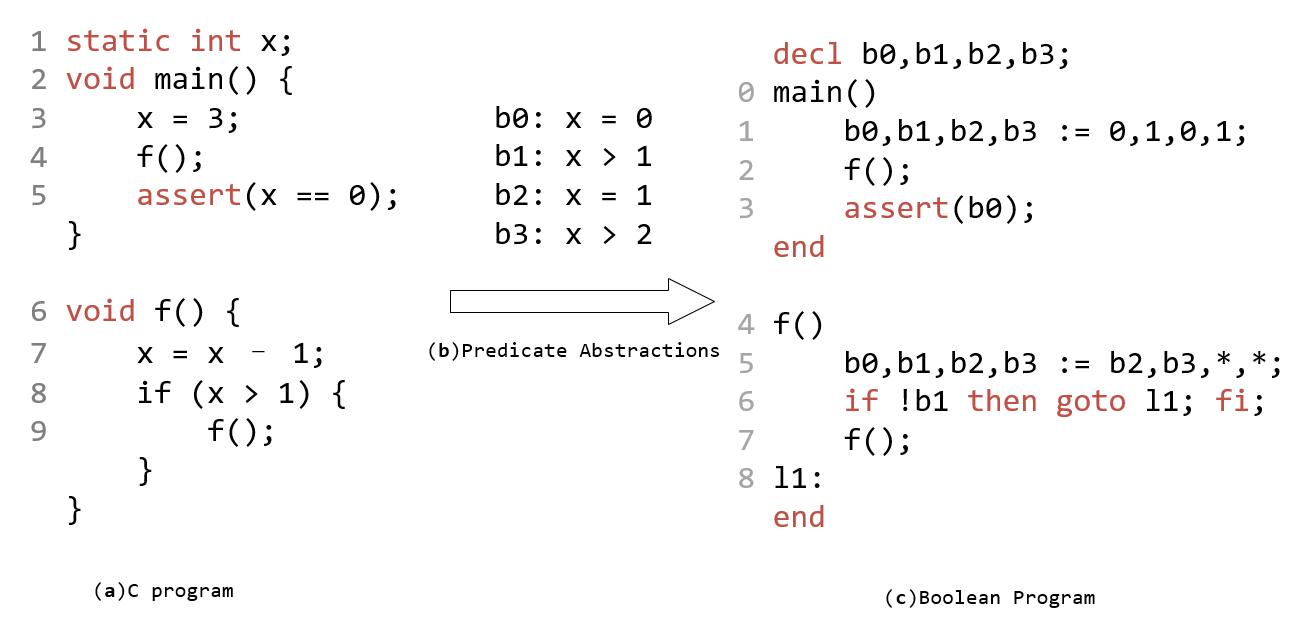
\includegraphics[width=5in,height=2.5in]{img/Fig2-1.jpg}
\caption{An example of boolean program conversion}
\label{fig:BPC}
\end{figure}

\begin{figure}
\centering
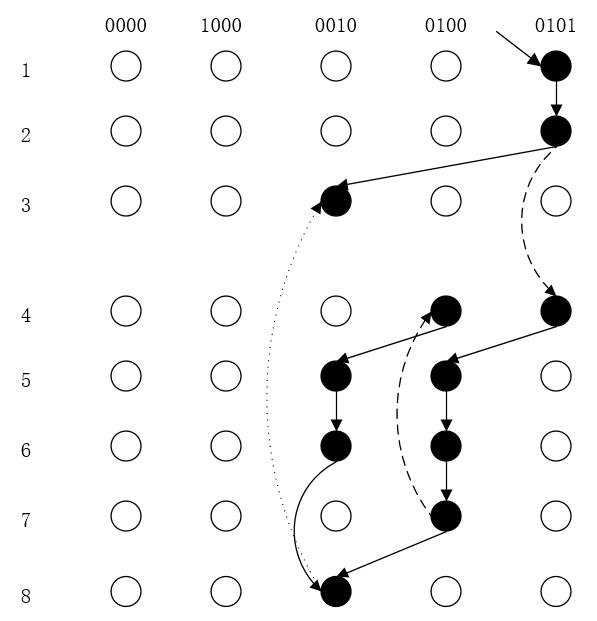
\includegraphics[width=2.5in,height=2.5in]{img/Fig2-2.jpg}
\caption{The control flow graph}
\label{fig:CFG}
\end{figure}

Takes Figure \ref{fig:BPC} as an example. For the C program in Figure(a), it is obvious that the assertion in line 5 cannot be satisfied. By abstracting the C program using the predicates in Figure(b), the program can be converted to the boolean program in Figure(c). The corresponding control flow graph is shown in Figure \ref{fig:CFG}. Note that the value combinations for $b0$, $b1$, $b2$ and $b3$ can only be $0000$, $1000$, $0010$, $0100$ or $0101$.

\subsection{Constructing Boolean Program}
\label{section:ConstructingBooleanProgram}
% 本文中用于代码修复的布尔程序是通过SATABS对C程序转换得来的。
The boolean program used for program repair in this paper is converted from C program by using SATABS\cite{SATABS}.
% SATBS是一个模型检测的工具,实现了谓词抽象细化循环,它能够将C/C++的程序转换成布尔程序。
SATABS, being a useful tool for model checking, implements iterative predicate abstraction refinement algorithm\cite{CCoCaVUPAaI}, and can be used to convert ANSI-C program to an equivalent boolean program.
% 给定了输入程序之后,SATABS会自动计算出它的抽象表示。为了达到程序的状态空间缩减的目的,抽象是一个很有效的方法。
For a given C program, SATABS will compute for its abstract representation automatically, which is an effective way to reduce the number of states.
% 谓词抽象是其中一种广泛应用的方法,它通过只保持跟踪一定的谓词来抽象数据。在抽象模型中,消去了原程序的变量,以布尔变量来表示根据原程序抽象出来的谓词
Predicate abstraction\cite{CoASGwPVS,GFSAoRSUDP} is one of the most popular abstracting algorithms, which abstracts the program's data by tracking a limited number of predicates.
% 在抽象模型中,消去了原程序的变量,以布尔变量来表示根据原程序抽象出来的谓词。
In the abstract model, variables of the original program will be omitted, and boolean variables will be used to represent the abstracted predicates.
% 抽象程序是通过存在抽象创建的,存在抽象对于可达性属性来说是保守的抽象,也即对于在抽象模型中存在的属性,也一定能在原始程序中找到同样的属性。
% The abstracted program is produced by existential abstraction\cite{MCaA}, which is a pretty conservative abstraction for reachability properties, meaning for every property in the abstracted model, there will always be a corresponding property in the original program.
\subsubsection{Converting an Assignment Statement}
\label{section:ConvertingAnAssignmentStatement}
% SATABS根据具体程序的状态迁移关系计算基本块的抽象迁移关系,得出抽象谓词集合P,每一个布尔变量对应集合P中的一个谓词。
Based on the state transitions of the given program, SATABS can calculate the abstracted state transitions between basic blocks and produce a set of abstracted predicates $P$, with every boolean variable corresponds to one predicate in $P$.
% 在得出谓词集合后进行转换的过程中,若原始程序在位置L处有赋值语句x=e,则布尔程序B在L出将包含对布尔变量的赋值语句[6]。
When the program is being converted, if there used to be an assignment statement, for example $x = e$, at location $L$ in the original program, there will also be an assignment statement for the corresponding boolean variable at location $L$ in the boolean program\cite{MLS:STEPaBP}.
% 布尔变量的真假值根据计算出的抽象状态迁移关系的谓词的真假值进行复制。
Value for the boolean variable is computed based on its corresponding predicate.
% 如果在L处不能确定谓词的真假值,则在B中的布尔变量只表示为:b_i= *。
If the value of the predicate cannot be determined at location $L$, the statement in $B$ will look like $b_{i} = *$, meaning {\it uncertain}.

For example, given the C program in Figure \ref{fig:BPC}(a), the predicate set computed by SATABS is $\{b0 : x = 0, b1 : x > 1, b2 : x = 1, b3 : x > 2\}$. Then it is easy to know the boolean assignment statements for C statements $x = 3$ and $x = x - 1$ will be $b0,b1,b2,b3 := 0,1,0,1$ and $b0,b1,b2,b3 := b2,b3,*,*$.

\subsubsection{Converting a Control Flow Statement}
\label{section:ConvertingAControlFlowStatement}
% 除了由赋值语句组成的初始块,程序中还包括了if、while和for等控制语句。
Except for basic blocks of assignment statements, there are also control flow statements like \lstinline|if|, \lstinline|while| and \lstinline|for| in boolean program.
% 这些语句包含作为参数的条件语句,但它们不会改变变量的取值而只会决定控制流的方向 \cite{35}。
Some of them can have conditional expression as their parameter, but they will not change the values of variables: all they do is changing the direction of control flow.
% 表2-1中给出了C语言程序中比较常见的控制语句转换的例子。从表中的3个例子可以总结出C语言程序的控制结构转换为布尔程序的规则。
Table \ref{table:ControlStatementConversions} shows examples of conversions of $C$ control flow statements, one can easily sum up the basic rules behind these conversions by these examples.

\begin{table}
\label{table:ControlStatementConversions}
\center
\caption{Examples of Boolean Statement Conversions}
\begin{tabular}{c|l|c|l}
\hline
Type & C & Predicate & Boolean Program \\
\hline
(1)$if$&
\begin{lstlisting}
if(x>1){
  f();
}
\end{lstlisting}&
\begin{lstlisting}
b1 : x>1
\end{lstlisting}&
\begin{lstlisting}
  if !b1
  then
    goto l1;
  fi;
  f();

l1:
\end{lstlisting} \\
\hline
(2)$while$&
\begin{lstlisting}
while(x>1){
  x=x-1;
}
\end{lstlisting}&
\begin{lstlisting}
b0 : x==0
b1 : x>=1
b2 : x==1
b3 : x>=2
\end{lstlisting} &
\begin{lstlisting}
l1:
  if !b2
  then
    goto l2;
  if;
  b0,b1,b2,b3 :=
      b2,b3,*,*;
  goto l1;
l2:
\end{lstlisting} \\
\hline
(3)$for$&
\begin{lstlisting}
a=2;
for(i=0;i<a;i++){
  x=x-1;
}
\end{lstlisting} &
\begin{lstlisting}
b0 : x==0
b1 : i>=a
b2 : 1+i>=a
b3 : x==1
b4 : a<=0
b5 : a<=1
\end{lstlisting} &
\begin{lstlisting}
  b1,b2,b4,b5 :=
    *,*,0,0;
  b1,b2 := b4,b5
l1:
  if b1
  then
    goto l2;
  if;
  b0,b3 := b3,*;
  b1,b2 := b2,*;
  goto l1;
l2:
\end{lstlisting} \\
\hline
\end{tabular}
\end{table}

% 对于if条件选择,我们假设原始C语言程序在位置L对一个控制条件语句进行判断:如果该控制条件成立,那么程序将会跳转到位置L_T继续执行条件成立时的语句,否则会跳转到位置L_F执行该条件不成立时的语句。
For conditional statement \lstinline|if|, we assume there is such an \lstinline|if| statement at location $L$, evaluating a boolean expression: if the expression is \lstinline|true|, the control flow goes to location $L_{T}$, otherwise it goes to $L_{F}$.
% 转换时,我们需要对控制条件语句进行抽象,首先就需要遍历该语句的语法结构,检查该控制条件语句中的子表达式是否是谓词集合P中的谓词:
During the conversion, we need to abstract the boolean expression. First of all we need to scan the syntactic structure of this expression, examining whether the sub-expressions belong to predicate set $P$:
% 如果是的话,用对应的布尔变量b_i取代控制条件语句中的表达式。
if they are, we replace the sub-expressions with their corresponding boolean variables $b_{i}$.
% SATABS所采用的策略是对转换后的控制条件语句c进行取非,真正在布尔程序中用于判断的条件语句为c:当c成立时,程序将会跳转到位置L_F,即例子(1)中的l1,并结束if表达式;否则,程序将进入位置L_T,即例子中if语句的后续语句,继续执行。
What SATABS does is negating the converted boolean expression $c$: the exact expression that is used in the converted program would be $\overline{c}$. If $\overline{c}$ is \lstinline|true|, the program will go to location $L_{F}$, being the \lstinline|l1| in example (1), and ends the \lstinline|if| statement; otherwise, the program will go to location $L_{T}$, being the statements right after the \lstinline|if| statement in the example.

% while条件循环语句在布尔程序中则被转换成了if条件选择。
As for \lstinline|while| loop, they are converted into \lstinline|if| statements in boolean program.
% 假设原式C语言程序在位置L有一个对条件语句c进行判断的while条件循环语句,转换后的表达式遵循如下规则:若c不成立,程序将跳转到位置L_F;否则,程序跳转至位置L_T,执行完循环体对应的所有语句后重新跳转到位置L。
As usual, we assume there is a \lstinline|while| statement at location $L$ in the original program, evaluating boolean expression $c$. The converted statement follows such rule that: if $c$ is \lstinline|false|, the program will goto location $L_{T}$, exiting the \lstinline|while| loop; otherwise, the program goes to location $L_{T}$, execute the body of the loop, and goes back to location $L$ for the next loop.

% for条件循环语句在布尔程序中同样被转换成了if条件选择。
\lstinline|for| loops are also converted into \lstinline|if| statements in boolean program.
% 本质上,while循环与for循环是相同的,差别仅在于for循环能够同时为循环内部声明局部变量,因此也需要对其所声明的局部变量进行抽象。
Essentially, \lstinline|for| loop and \lstinline|while| loop are similar, the difference is one can declare local variables in the initialization of \lstinline|for| loop, being the variable \lstinline|i| in example (3). Hence, it is necessary for us to abstract these local variables.
% 转换时,for循环的初始化语句被转换为对应的赋值语句后,放在了转换后的if语句的上方。
The initialization of the original \lstinline|for| loop will be placed above the converted \lstinline|if| statement,
% 同时,for循环的增量表达式也被转换为了赋值语句,并被置于标志循环体结束的goto语句上方。
while the afterthought being converted into assignment statement and placed above the \lstinline|goto| statement, which stands for the end of the loop body.

\subsubsection{Converting a Function Invocation}
\label{section:ConvertingAFunctionInvocation}
% 布尔程序对于原始C语言程序中的函数调用将进行保留,因此布尔程序可以很好地展现具体的C语言程序里的函数调用关系。
Converted boolean program will reserve the function invocations from the original $C$ program, by which the boolean program can reflect the correlations of functions in the original $C$ program accurately.
% 函数的调用分为有参数与无参数函数调用,以及有返回值与无返回值函数调用,其中有参数和无参数的函数调用在转换为布尔程序后均被转化为了无参数函数调用。
For $C$ language, there are invocations with and without parameters, and also functions with and without result returned. For parameter, all functions will be converted into its no-parameter equivalence in boolean program.

% 对于无返回值函数的调用,一般情况下被调用函数都是用于对全局变量进行操作,因此函数调用语句本身可以直接转换,即无论函数调用语句是f()还是f(x),转换成布尔程序后均为f()。
For invocation of function with no result returned (\lstinline|void| function), generally such function will only be used to manipulate global variables, hence it would be equivalent to convert them all to invocation of function without parameter, meaning whether they are \lstinline|f()| or \lstinline|f(x)| in the original program, they will all be \lstinline|f()| in the converted boolean program.

% 对于有返回值函数的调用则稍微复杂一些。在转换时,我们需要额外声明一个布尔变量:该布尔变量不表示任何从C语言程序中抽象出来的具体谓词,而是用于表示被调用函数的返回值。
It would be a little tricky when we are dealing with functions with result returned. During the conversion, we need to declare such a boolean variable additionally: it does not stand for any predicates abstracted from the original variables in the $C$ program, but only stands for the returned result of the invoked function.

\begin{figure}
\centering
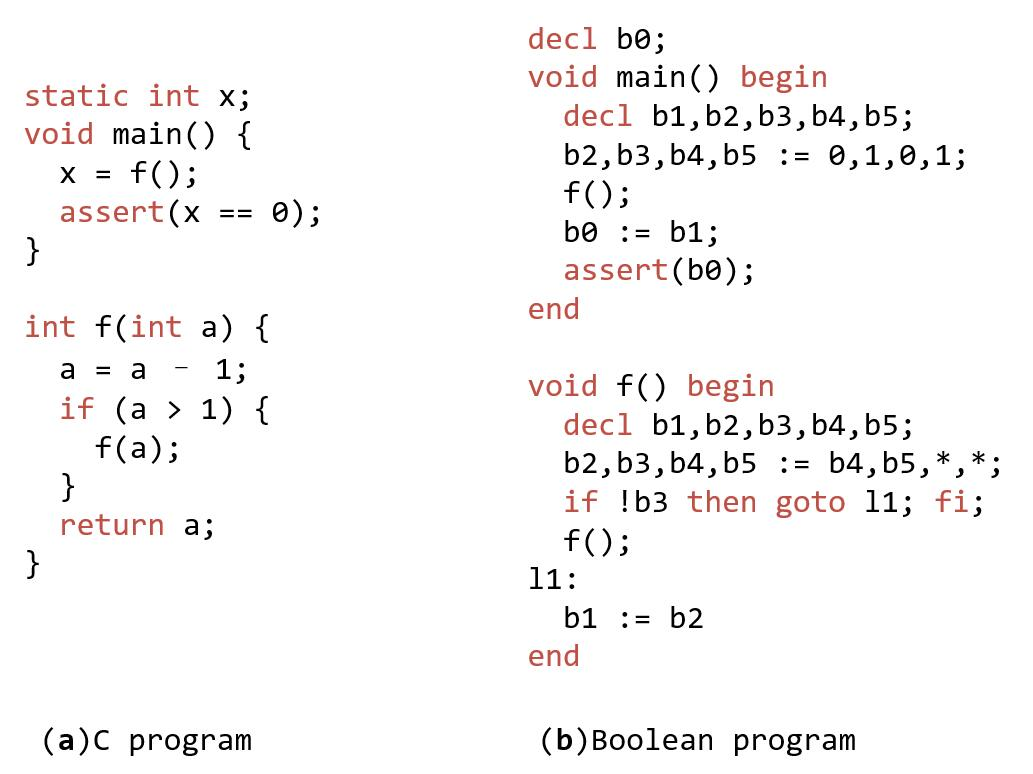
\includegraphics[width=4in,height=3in]{img/Fig2-3.jpg}
\caption{Another example of boolean program conversion}
\label{fig:BPC_1}
\end{figure}

% 如图2-3中所示的布尔程序,变量b_1代表的便是被调用函数f的返回值。
Figure \ref{fig:BPC_1} shows an example boolean program, in which variable \lstinline|b1| stands for the result returned by function \lstinline|f|.
% 进行函数调用的时候,在调用语句之前,程序会对被调用函数里的局部变量赋初始值,在被调用函数结尾会将返回值赋予该布尔变量,并在调用语句结束后将该布尔变量的值赋予赋值语句所指定的布尔变量。
Before the invocation statement, the converted program will initialize the local variables declared in the invoked function's body, and assign the returning result to the additionally-declared variable at the end of the body.

\subsection{Conjunctive and Disconjunctive Normal Form}
\label{section:CNF_DNF}
In mathematical logic, a \textit{well-formed formula}, often simply \textit{formula}, is a word (i.e. a finite sequence of symbols from a given alphabet) that is part of a formal language.
The formulas of propositional calculus, also called propositional formulas\cite{FOLaATP}, are expressions such as $(A \wedge (B \vee C))$. Their definition begins with the arbitrary choice of a set $V$ of propositional variables. The alphabet consists of the letters in V along with the symbols for the propositional connectives and parentheses "(" and ")", all of which are assumed to not be in V. The formulas will be certain expressions (that is, strings of symbols) over this alphabet.

The formulas are inductively defined as follows:
\begin{itemize}
\item Each propositional variable is, on its own, a formula.
\item If $\varphi$ is a formula, then $\neg \varphi$ is a formula.
\item If $\varphi$ and $\psi$ are formulas, and $\bullet$ is any binary connective, then $\varphi \bullet \psi$ is a formula. Here $\bullet$ could be (but is not limited to) the usual operators $\vee$, $\wedge$, $\to$, or $\leftrightarrow$.
\end{itemize}

In Boolean logic, a formula is in \textit{conjunctive normal form} (CNF) if it is a conjunction of clauses, where a clause is a disjunction of literals; otherwise put, it is an \textit{AND} of \textit{OR}s.
As comparison, a \textit{disjunctive normal form} (DNF) is a standardization (or normalization) of a logical formula which is a disjunction of conjunctive clauses, which can also be described as an \textit{OR} of \textit{AND}s.
For conjunctive and disconjunctive normal form, the only propositional operators are \textit{and}($\wedge$), \textit{or}($\vee$) and \textit{not}($\neg$), where the \textit{not} operator can only be used as part of a literal, meaning it can only precede a propositional variable.

The formal grammar for DNF and CNF can be expressed as follows:

\begin{tabular}{ccc}
$\textit{literal}$ & $\to$ & $\textit{variable}$ \\
$\textit{literal}$ & $\to$ & $\neg \textit{variable}$ \\
$\textit{conjunctive clause}$ & $\to$ & $\textit{literal}$ \\
$\textit{conjunctive clause}$ & $\to$ & $(\textit{literal} \wedge \textit{conjunctive clause})$ \\
$\textit{DNF}$ & $\to$ & $\textit{conjunctive clause}$ \\
$\textit{DNF}$ & $\to$ & $(\textit{conjunctive clause} \vee \textit{DNF})$ \\
$\textit{disjunctive clause}$ & $\to$ & $\textit{literal}$ \\
$\textit{disjunctive clause}$ & $\to$ & $(\textit{literal} \vee \textit{disjunctive clause})$ \\
$\textit{CNF}$ & $\to$ & $\textit{disjunctive clause}$ \\
$\textit{CNF}$ & $\to$ & $(\textit{disjunctive clause} \wedge \textit{CND})$
\end{tabular}

where \textit{variable} can be any variable.

\subsection{Satisfiability Modulo Theories}
\label{section:SatisifiabilityModuloTheories}
Variables in converted boolean program are somehow different from general boolean variables: they all are bound to specific predicates abstracted from the original $C$ program, which provide them {\it meanings}.
With all these meanings behind them, some value combinations would be impossible for them to take, as such combinations result in conflicts on their meanings.
For example, consider a predicate abstraction where $p_{1}$ stands for \lstinline|x == 0| and $p_{2}$ stands for \lstinline|x == 1|.
Combination \lstinline|p1 : true, p2 : true| is impossible as it is impossible for \lstinline|x == 0| and \lstinline|x == 1| both being \lstinline|true| at the same time.
It is important to consider which combinations are possible for a boolean program, as the set of all possible combinations would be generally smaller than $2^{V}$.
Considering other problems in a smaller set can bring great reduction to the search space.
Hence, we introduce satisfiability modulo theories.

In computer science and mathematical logic, the satisfiability modulo theories (SMT) problem\cite{SMT} is a decision problem for logical formulas with respect to combinations of background theories expressed in classical first-order logic with equality.
Formally speaking, an SMT instance is a formula in first-order logic, where some function and predicate symbols have additional interpretations, and SMT is the problem of determining whether such a formula is satisfiable.
In other words, SMT problem can be considered as a SAT\footnote{Boolean satisfiability problem} problem in which some of the binary variables are replaced by predicates over a suitable set of non-binary variables\cite{BSAT:SMT}.

We assume a countable set of variables $X$, function symbols $F$ and predicates $P$.\cite{ToSMT}
A first-order signature $\Sigma$ is a partial map from $F \cup P$ to the natural numbers corresponding to the {\it arity} of the symbol.
A $\Sigma$-{\it term} $\tau$ has the form
\begin{equation}
\label{eq:SigmaTerm}
\tau := x | f(\tau _{1}, \dots, \tau _{n})
\end{equation}
where $f \in F$ and $\Sigma(f) = n$. For example, if $\Sigma(f) = 2$ and $\Sigma(g) = 1$, then $f(x, g(x))$ is a $\Sigma$-term.
A $\Sigma$-{\it formula} has the form
\begin{equation}
\label{eq:SigmaFormula}
\psi := p(\tau _{1}, \dots, \tau _{n}) | \tau _{0} = \tau _{1} | \neg \psi _{0} | \psi _{0} \vee \psi _{1} | \psi _{0} \wedge \psi _{1} | (\exists x : \psi _{0}) | (\forall x : \psi _{0})
\end{equation}
where $p \in P$ and $\Sigma(p) = n$, and each $\tau _{i}$ is a $\Sigma$-term. For example, if $\Sigma(<) = 2$ for a predicate symbol $<$, then $(\forall x : (\exists y : x < y))$ is a $\Sigma$-formula.
A $\Sigma$-{\it structure} $M$ consists of a nonempty domain $|M|$, for each $p \in P$ such that $\Sigma(p) = n$, $M(p)$ is a subset of $|M|^{n}$, and for each $x \in X$, $M(x) \in |M|$.
The interpretation of a term $a$ in $M$ is given by $M\llb x \rrb = M(x)$ and $M\llb f(a_{1},\dots,a_{n})\rrb = M(f)(M\llb a_{1}\rrb\dots M\llb a_{n}\rrb )$.
For a $\Sigma$-formula $\psi$ and a $\Sigma$-structure $M$, satisfaction $M \models \psi$ can be defined as

\emptyline
\begin{center}
\begin{tabular}{rcl}
$M\models a = b$                      & $\Longleftrightarrow$ &   $M\llb a\rrb = M\llb b\rrb$                            \\
$M\models p(a_{1},\dots,a_{n})$       & $\Longleftrightarrow$ &   $(M\llb a_{1}\rrb,\dots,M\llb a_{n}\rrb) \in M(p)$     \\
$M\models\neg\psi$                    & $\Longleftrightarrow$ &   $M\not\models\psi$                                     \\
$M\models \psi _{0}\vee\psi _{1}$     & $\Longleftrightarrow$ &   $M \models\psi _{0}$ or $M\models\psi _{1}$            \\
$M\models \psi _{0}\wedge\psi _{1}$   & $\Longleftrightarrow$ &   $M\models\psi _{0}$ and $M\models\psi _{1}$            \\
$M\models (\forall x : \psi)$         & $\Longleftrightarrow$ &   $M\{x\mapsto a\}\models\psi$, for all $a\in |M|$       \\
$M\models (\exists x : \psi)$         & $\Longleftrightarrow$ &   $M\{x\mapsto a\}\models\psi$, for some $a\in |M|$      \\
\end{tabular}
\end{center}
\emptyline

A first-order $\Sigma$-formula $\psi$ is {\it satisfiable} if there is a $\Sigma$-structure $M$ such that $M \models\psi$, and it is valid if in all $\Sigma$-structures $M$, $M \models\psi$.
\newpage

\section{Boolean Program Repair}
\label{section:BooleanProgramRepair}
\subsection{Repairing by Bad Routes}
% 为了找到错误,首先要建立合适的错误模型。在本文中,我们假设程序只包含一个错误,也就是说在C 语言程序中只包含一个错误语句。
To locate fault accurately, establishing an appropriate model of {\it fault} is essential. In the following sections, we assume there is only one line of faulty code in the original $C$ program.
\subsubsection{Constructing Fault Model}
% 本文的错误模型只针对C语言程序的一个语句,更确切的说是针对C语言程序里的一行语句。
In this paper, we focus on one single error in the original $C$ program. To be more specific, one {\it line} of faulty statement is all we concern.
% 在转换为布尔程序的过程中,原C语言程序的一个变量可能会对应多个布尔变量,C语言程序的一行也可能对应布尔程序的多行,而本文在对转换后的程序进行修复也只是针对布尔程序的一行错误进行修复。
After being converted to boolean program, one variable in $C$ program can correspond to multiple boolean variables, one line of statement can also be converted into multiple lines of statements in boolean program,
but only those kinds of errors that maps to one single line of statement in boolean program we try to achieve automatic repair.
% 因此本文的错误模型在转换为布尔程序后对应的错误模型也必须只体现在一行语句上。
Thus, the fault model used in this paper can only be applied to one single line of statement after being converted to the corresponding fault model for boolean program.
% 形式化来讲,我们的错误模型有定义如下:
Formally speaking, our fault model can be defined as follows:
\begin{definition}
% 当C语言程序的出错语句为控制语句c的控制条件时,则对应的布尔程序中出错的语句为控制语句c_b;
If there is a fault in the conditional expression of the control flow statement $c$ in the original $C$ program, the corresponding faulty statement in the boolean program is control flow statement $c_{b}$;
% 当C语言程序出错的语句为赋值语句s时,则对应的布尔程序中出错的语句为赋值语句s_b。
if the fault is in the $C$ assignment statement $s$, the corresponding fault is in the boolean assignment statement $s_{b}$.
% 即C语言程序的单行错误语句映射到布尔程序的单行错误语句。
In a word, one line of faulty statement in $C$ will only correspond to one line of faulty statement in boolean program.
\end{definition}

\begin{figure}
\centering
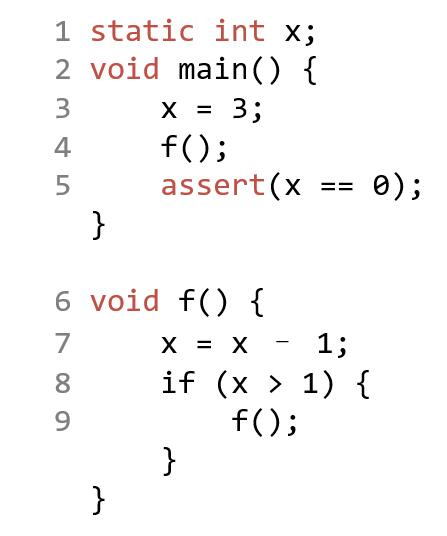
\includegraphics[width=1.7in,height=2in]{img/Fig3-1.jpg}
\caption{The C program from Figure \ref{fig:BPC}}
\label{fig:FC}
\end{figure}

% 我们将图2-1(a)作为图3-1。在这个错误的C语言程序中,变量x在程序启动时被赋予了初值3,并且程序在完成对函数f的调用后,使用语句assert(x==0)对程序的当前状态进行了断言。
We used Figure \ref{fig:BPC}(a) again, as Figure \ref{fig:FC}. In this faulty $C$ program, variable \lstinline|x| is initialized as \lstinline|3|, and the program uses statement \lstinline|assert(x == 0)| to assert its state after the invocation of function \lstinline|f|.
% 实际上,这两个操作组成了单元测试用例的两个主要元素,即“将程序设置到某个特定的状态”以及“断言程序的最终状态”。
Actually, such operations make up the two basic elements of unit test case, which are "setting the program to a specific initial state" and "asserting the program's final state", or "a known input" and "an expected output" if you prefer.
% 我们给出错误程序的定义:
Here, we give out the basic definition of a faulty program:

\begin{definition}
\label{definition:FaultyProgram}
% 对于布尔程序B,若给定的初始状态使得B在某个assert语句上断言失败,那么我们就说B没能通过由该初始状态和assert语句所断言的最终状态组成的单元测试,即布尔程序B是错误的。
For boolean program $B$, if a given initial state makes $B$ fail to pass some \lstinline|assert| statements, then we say program $B$ doesn't pass the unit test case made up of this initial state and \lstinline|assert| statement,
meaning program $B$ has a fault.
\end{definition}

Also, the definition of a correct program is pretty intuitive:

\begin{definition}
\label{definition:CorrectProgram}
% 正确的程序在运行的过程中总能从初始状态走到程序的正确终止状态且不会经过会使断言失败的错误状态。
A {\it correct} program can always walk from initial state to expected termination state, without passing any wrong state that makes an assertion failed.
\end{definition}

% 在2.1节中,我们将布尔程序的运行图视为了一个有穷自动机。在有穷自动机中,“路径”的概念自然是不陌生的。那么,对于这样的有穷自动机,我们不妨得出其路径的定义如下:
In section \ref{section:SyntaxAndSemanticsOfBooleanProgram}, we describe the control graph of boolean program as a DFA\footnote{Deterministic finite automaton}. No doubt the concept of "path" for DFA should be familiar. In that sense, we define the path of such boolean program DFA as follows:

\begin{definition}
A {\it route} $r$ of boolean program $B$ is an ordered sequence of states $Q_{r}=(q_{r}^{(0)},q_{r}^{(1)},\dots,q_{r}^{(t)})$, in which for any pair of elements $q_{r}^{(i)}$ and $q_{r}^{(i + 1)}$ that makes $i \ge 0$, we have $next(q_{r}^{(i)}) = q_{r}^{(i + 1)}$. In the control graph, a route is represented by a sequence of end-to-end connected edges.
\end{definition}

% 结合定义3.2和定义3.3,我们给出错误路径的定义
With definition \ref{definition:FaultyProgram} and \ref{definition:CorrectProgram}, the definition of bad route can be described as follows:

\begin{definition}
For a route $r$, if there is such state $q_r^{i} = (s,\xi)$ that statement $s$ is an assertion statement and the current evaluation $\xi$ doesn't satisfy this assertion, we say route $r$ is a {\it bad} route.
\end{definition}

\subsubsection{Collecting Bad Routes}
\label{section:CollectingBadRoutes}
% 对于已知的错误语句,我们需要计算出正确的修复语句来进行替换。
For a located faulty statement, we need to produce a correct repairing statement to replace it.
% 我们假设*rep是任意与变量相关的函数,并将*rep作为替换错误语句的表达式,即修复语句。
Assume $*rep*$ is an arbitrary function of all boolean variables, and consider $*rep$ (or the invocation of it) as the repairing statement.
% 替换后,我们便需要去考虑在替换出所延伸出的每种可能路径。
After the replacement, the concrete implementation of $*rep$ is still unknown, hence we need to consider every possible route branches off at this point.

% 假设布尔程序B中只出现了一个*rep。为了计算*rep的恰当实现,我们需要构造该程序的状态转移图。
Assume there is only one $*rep$ in the boolean program $B$. To produce the appropriate implementation of $*rep$, we need to re-construct the state transition graph of this program and every routes branch off at this point
that might lead to wrong termination state.
% 在*rep出现的地方,可以根据它的一个实现从当前状态转移到下一个状态,而它不同的实现则会使当前状态迁移到不同的状态。
When we confronts $*rep$, we can move from one state to another based on one of its possible implementations, and different implementations lead to different states.

% 假设有估值集合,满足:
An implementation of $*rep$ can be considered as a mapping from evaluation to a boolean value (the result of $*rep$). Assume we have a set of evaluations $c \subseteq X$, which satisfies:
\begin{definition}
For any $\xi \in X$, $*rep(\xi) = 1$ if and only if $\xi \in c$. $C = 2^{c}$ is the set of all implementations of $*rep$.
\end{definition}
In other word, $c$ is the set of evaluations which makes $*rep$ return $1$. For each $c$, it would be easy to imagine its corresponding $*rep$ implementation (the mapping).

\begin{figure}
\centering
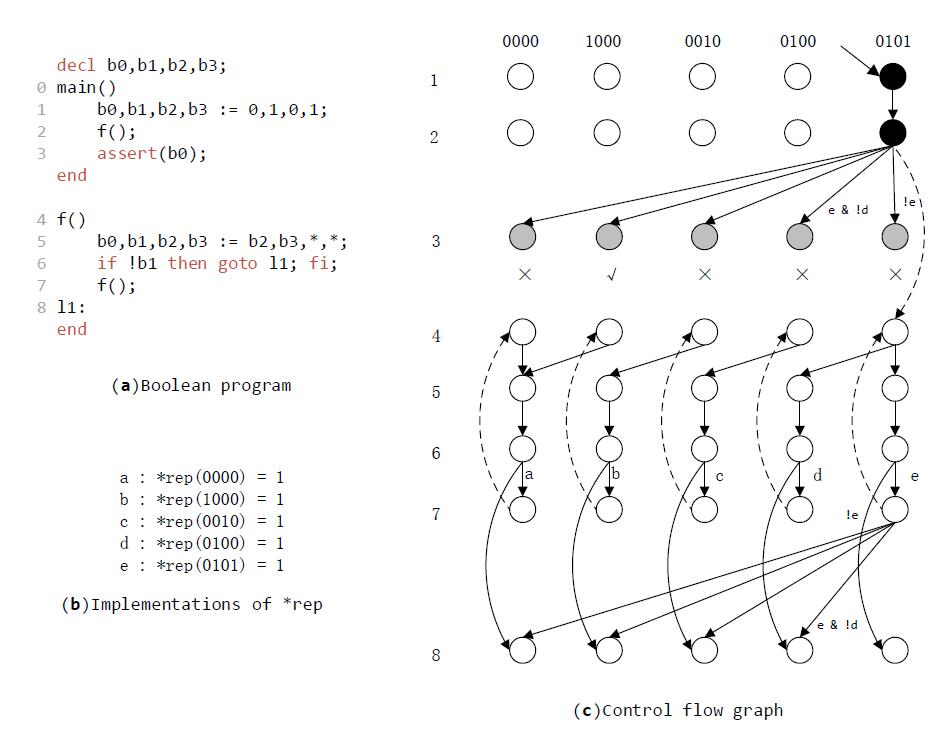
\includegraphics[width=5in,height=3.5in]{img/Fig3-2.jpg}
\caption{An example of finding all bad routes}
\label{fig:FBR}
\end{figure}

Takes Figure \ref{fig:FBR} as an example, where Figure(a) is basically the same as Figure \ref{fig:BPC}(b).
After replacing the faulty statement with $*rep$, by considering every possible transition corresponding to different $*rep$ implementations,
one can easily draw the control flow graph in \ref{fig:FBR}(c). In this example, we give out predicates $a$, $b$, $c$, $d$ and $e$, representing different elements in evaluation set $c$.
% 以状态(6,00111)为例,程序在此行对*rep函数返回的结果进行判断:若此时函数返回1,即命题e成立,程序进入状态(7,00111)并再次调用函数f;反之,若此时函数返回0,即命题e不成立,程序进入状态(8,00111)并结束函数f。
For example, in state $(6,0101)$, the program will examine the result of function $*rep$: if the function return $1$, meaning predicate $e$ is satisfied, the program will result in state $(7,0101)$ and invoke function \lstinline|f| again; otherwise, if predicate $e$ cannot be satisfied, the program will result it state $(8,0101)$ and return from function \lstinline|f|.
% 假设我们进入了状态(7,00111)并随之来到了状态(6,00110),程序再次对*rep函数返回的结果进行判断:若此时函数返回0,即命题d不成立,程序进入状态(8,00110)并结束函数f。
Assume we enter state $(7,0101)$ and then state $(6,0100)$, the program will examine the result of function $*rep$ again: if the function return $0$, meaning predicate $d$ is unsatisfied, the program will enter state $(8,0100)$ and return from function \lstinline|f|.
% 依此类推,我们就可以计算出main函数从状态(2,00111)分别进入到第三行五个不同状态所需满足的条件。其中,状态(3,10000)、(3,00100)、(3,00110)、(3,00111)均无法通过断言,属于错误状态,其所属的路径便是错误路径。
By repeating this, one can calculate the different requirements for the program to enter the 5 different states in line $3$. Among them, state $(3,0000)$, $(3,0010)$, $(3,0100)$ and $(3,0101)$ cannot pass the assertion, meaning they are wrong termination states, and the routes they belong to are bad routes.

\subsubsection{Producing Repairing Statement}
\label{section:ProducingRepairingStatement}
% 前文的过程可以找到状态转移图中所有连接初始状态和错误终止状态的错误路径。
By constructing all possible routes that lead the program into wrong termination states, we actually find out all wrong implementations of $*rep$.
% 那么不难得出,*rep的正确实现则是这些错误实现所组成的集合的补集。
Then it would be intuitive to know the correct implementation of $*rep$ is the complementary of all these wrong implementations.

\begin{definition}
\label{definition:CorrentREP}
Assume for every implementation $c$ of $*rep$ there is a concrete execution route $r_{c}$, the correct implementation of $*rep$ is $I = C - \{c | \exists q \in r_{c} \wedge q \in bad\}$, where $bad$ is the set of all wrong states.
\end{definition}

% 在上述例子中,我们便收集到了状态(3,10000)、(3,00100)、(3,00110)、(3,00111)所对应的四个错误的*rep实现 ...,即当*rep的实现满足...时,程序将从初始状态进入错误的终止状态。
In the above example, we collect four wrong implementations of $*rep$ corresponding to states $(3,0000)$, $(3,0010)$, $(3,0100)$ and $(3,0101)$: $bcde$, $\cap{c}de$, $\cap{d}e$ and $\cap{e}$,
meaning if the implementation of $*rep$ satisfies $bcde \vee \cap{c}de \vee \cap{d}e \vee \cap{e} = b \vee \cap{c} \vee \cap{d} \vee \cap{e}$, the program will enter wrong state.
% 根据上述定理,我们可以得出正确的*rep实现...,即唯一一条走向正确终止状态(3,01000)的路径。
Based on the above definition, one can safely produce the correct implementation of $*rep$, being $I = \cap{b}cde$, which is also the only route that leads to the correct termination state $(3,1000)$.
% I转换为为此表示并化简后,可得结果...
After representing $I$ with the corresponding predicates and simplifying it based on first-order logic simplification rules, we have $I = \neg b_{0}$.

\subsection{The Satisfiability of the Repairing Statement}
\label{section:TheSatisfiabilityOfTheRepairingStatement}
% 在得出修复公式后,我们还需要考虑该公式是否是可满足的。
After producing the repairing statement, we also need to consider if this statement is satisfiable.

% 布尔程序是对C程序抽象而来,得到布尔程序的修复之后,需要将其重新转换为C语言的修复语句。
Boolean program is abstracted from the original $C$ program. After producing the repairing statement, we also need to convert it back to the corresponding $C$ statement.
% 布尔程序的修复公式,简称布尔修复,是由一系列布尔变量和操作符构成的布尔表达式,其中的布尔变量由C语言程序转换为布尔程序中对原有的变量进行谓词抽象所得,因此布尔修复的每个布尔变量都有着对应的谓词。
The repairing statement for the boolean program, or {\it boolean repair}, is a boolean expression consists of boolean variables and operations, in which all boolean variables are produced by predicate abstraction of the original $C$ program, meaning every boolean variable in the boolean repair has its corresponding predicate.
% 我们应用上一节所述方法得出的布尔修复将会是一个一阶逻辑公式。
The boolean repair produced by the method described in the above section will be a first-order logic expression.
% 由于公式中的每个变量都着其背景理论,公式本身是否可满足是暂不确定的。
As every variable in the expression has its background theory, it is uncertain whether the expression itself is satisfiable.
% 例如图3-2中,谓词p_1的背景理论为x<0,谓词p_2的背景理论为x=0。考虑其背景理论后,实际上公式p_1∧p_2是不可满足的。
For example, in Figure \ref{fig:BPC}, the background theory of predicate $b_{0}$ is $x = 0$, while $b_{2}$ being $x = 1$. Expression $b_{0} \wedge b_{2}$ is clearly unsatisfiable after considering their background theories.
% 由此,我们必须在定义3.6的基础上细化对布尔修复的定义:
In this case, we need to refine the definition of boolean repair based on Definition \ref{definition:CorrentREP}:

\begin{definition}
% 设程序的所有错误路径集合为FP,且...是可满足的,则存在布尔修复使得程序正确,
Assume the set of all bad routes is $FP$, and $\neg (fp_{1} \vee fp_{2} \vee\dots fp_{n}$ is satisfiable, then we say there is a boolean repair that can repair the program.
% 该布尔修复为...,其中bad为程序所有错误状态所组成的集合。
The boolean repair is $I = C - \{c | \exists q \in r_{c} \wedge q \in bad\}$, where $bad$ is the set of all wrong states.
\end{definition}

% 由此,在布尔程序中找到修复公式并不代表能为原本的C语言程序找到修复表达式。
Therefore, existence of a repairing statement for boolean program does not necessarily mean the existence of a corresponding repairing statement for $C$ program.
% 而判断一阶逻辑公式在给定背景理论的情况下是否可满足的问题可以规约到可满足性模理论问题(SMT)
We need to determine if the boolean repair, being a first-order logic expression, is satisfiable after considering the background theories. Such problem can be reduced to the problem of SMT\footnote{Satisfiability modulo theories}\cite{SMT}.

% 我们不妨以析取范式来表示通过本文方法得出的布尔修复,即对于布尔修复φ_rep,有:
As the boolean repair is a first-order logic expression, it would be convenient to first convert it into disjunctive normal form, meaning if we have a boolean repair $\varphi _{rep}$, we have:
\begin{equation}
\varphi _{rep} = \varphi _{1} \vee \varphi _{2} \vee \dots \vee \varphi _{n}
\end{equation}
Every $\varphi _{i}$ is made up of predicate variables and has the following form:
\begin{equation}
\varphi _{i} := p(\tau _{i},\dots,\tau _{n}) | \varphi _{a} \wedge \varphi _{b}
\end{equation}
in which each term $\tau _{i}$ is a $\Sigma$-term (see Equation \ref{eq:SigmaTerm}), representing predicate abstracted from the original $C$ program.
In that sense, one can easily notice that the formula of $\varphi _{rep}$ satisfies the general form of $\Sigma$-formula (see Equation \ref{eq:SigmaFormula}).

% 此外,给定修复公式φ_rep有背景理论T_rep。
Additionally, we assume the background theories of $\varphi _{rep}$ is $T_{rep}$.
% 布尔程序的背景理论均由原C语言程序变量进行谓词抽象得出,因此背景理论T_rep对应修复φ_rep中的谓词变元p(τ_1,τ_2),背景理论的赋值模型与谓词变元的赋值模型一致。
The background theories of boolean program is abstracted from the original $C$ program, hence $T_{rep}$ corresponds to the predicate variable $p(\tau _{1}, \tau _{2})$ in $\varphi _{rep}$, having the same assignment model as predicate variable does.

% 综上,根据先前提到的对可满足性模理论问题的定义,可以证明修复公式φ_rep的可满足性问题都可以规约到可满足性模理论问题。
Above all, based on the definition of SMT shown in former section, one can prove the satisfiability problem of boolean repair $\varphi _{rep}$ can be reduced to SMT.
% 为布尔程序找到的修复公式一定是布尔程序的正确修复,而转换后的φ_rep是否能使C语言程序正确则仍需要进行可满足性判断。
The boolean repair produced by the method describe in the former section is actually the correct repairing statement for the boolean program, but the $\varphi _{rep}$ also has to be satisfiable after conversion.
For now, we know the satisfiability problem of boolean repair $\varphi _{rep}$ can be reduced to SMT, hence we can use the algorithm for SMT to solve the satisfiability program of $\varphi _{rep}$

\subsection{Boolean Repair Simplification}
\label{section:BooleanRepairSimplification}
% 给定析取范式φ,假设存在模型M使得...,即公式φ是可满足的。
For a given DNF\footnote{Disjunctive normal form} expression $\varphi$, assume there is such model $M$ that $M \models \varphi$, meaning expression $\varphi$ is satisfiable.
% 实际上,由于φ是一个析取范式,它的可满足性只能推出它包含可满足的合取子句,但并不能说明它的所有合取子句都是可满足的。
Actually, as $\varphi$ is a DNF expression, all can be inferred from its satisfiability is that it contains satisfiable conjunctive clause, it doesn't mean every clause of it is satisfiable.

% 形式化地说,对于给定的修复公式...,它的可满足并不代表每个φ_i都是可满足的。
Formally speaking, for a repairing statement $\varphi _{rep} := \varphi _{1} \vee \varphi _{2} \vee \dots \varphi _{n}$, it's satisfiability is not sufficient for the satisfiability of every $\varphi _{i}$.
% 例如,对于修复公式...。公式本身是可满足的,因为子句p_3可满足,但子句p_1∧p_2是不可满足的。
For example, consider an repairing statement $\varphi _{rep} := (p_{1} \wedge p_{2}) \vee p_{3}$, where $p_{1} : x > 2, p_{2} : x < 1, p_{3} : x = 0$. The expression is satisfiable as clause $p_{3}$ is satisfiable,
but clause $p_{1} \wedge p_{2}$ is unsatisfiable.

% 若将上例给出的修复公式转换为C语言表达式,我们可以得到C语言修复表达式x>2 && x<1 || x !=0,其中x>2 && x<1部分是没有意义的,该表达式可直接化简为x !=0。
If we convert the expression given in the example to $C$ statement, we have \lstinline{x > 2 && x < 1 || x != 0}, where \lstinline|x > 2 && x < 1| is meaningless, the statement can be simplified to \lstinline|x != 0|.
% 由此可见,我们在将布尔修复转换为C语言表达式前,还需要通过验证其各子句的可满足性来对其进行化简。
Hence, before we convert the boolean repair to $C$ statement, there will be ways to simplify the statement, removing unsatisfiable clauses is one of them.

% 接下来我们将通过三种不同的方式对公式进行化简。
In the following sections, we will use three different ways to simplify the repairing statement.

\subsubsection{Removing Unsatisfiable Clauses}
% 给定可满足的修复公式...,公式子句外的化简是通过判断公式中每个修复子句...的可满足性进行的。
For a given satisfiable repairing statement $\varphi _{rep} := \varphi _{1} \vee \varphi _{2} \vee \dots \vee \varphi _{n}$, one can proceed outer-clause expression simplification by examining the satisfiability of each clause $\varphi _{i}$.
% 如果修复子句φ_i是可满足的,则保留该修复子句;否则,则将其从修复公式φ_rep中移除。
If the clause is satisfiable, the clause should be preserved; otherwise, it can be removed from $\varphi _{rep}$.
% 由3.2节可知,判断子句的可满足性同样可以规约到可满足性模理论问题。
Based on section \ref{section:TheSatisfiabilityOfTheRepairingStatement}, the satisfiability problem of clause $\varphi _{i}$ can also be reduced to SMT.

% 我们将移除不满足修复子句后产生的新的修复公式称为φ_rep^'。
Assume the new repairing statement produced by removing all unsatisfiable clauses are $\varphi _{rep}'$.
% 可以证明,通过子句外化简得到的φ_rep^'和原修复公式φ_rep是等价的,即...。
One can prove $\varphi _{rep}'$ is equivalent to $\varphi _{rep}$, meaning $\varphi _{rep}' \Longleftrightarrow \varphi _{rep}$.

\begin{proof}
% 假设φ_rep^'由φ_rep移除不满足子句φ_i得出,即...
Assume $\varphi _{rep}'$ is produced by removing unsatisfiable clause $\varphi _{i}$ from $\varphi _{rep}$, meaning
\begin{equation}
\label{eq:1}
\varphi _{rep} = \varphi _{rep}' \vee \varphi _{i}
\end{equation}
It should be intuitive that
\begin{equation}
\varphi _{rep}' \Longrightarrow \varphi _{rep}' \vee \varphi _{i}
\end{equation}
Thus,
\begin{equation}
\varphi _{rep}' \Longrightarrow \varphi _{rep}
\end{equation}
We know clause $\varphi _{i}$ is unsatisfiable, meaning $\varphi _{i}$ is always $false$ and $\neg \varphi _{i}$ is always $true$. In this sense, we have
\begin{equation}
\neg \varphi _{i} \wedge (\varphi _{rep}' \vee \varphi _{i}) \Longrightarrow \varphi _{rep}'
\end{equation}
Based on equation (\ref{eq:1}), we have
\begin{equation}
\label{eq:2}
\neg \varphi _{i} \vee \varphi _{rep} \Longrightarrow \varphi _{rep}'
\end{equation}
Given the fact of $\neg \varphi _{i}$ always being $true$, we have
\begin{equation}
\neg \varphi _{i} \wedge \varphi _{rep} = \varphi _{rep}
\end{equation}
Combined with equation (\ref{eq:2}), we have
\begin{equation}
\varphi _{rep} \Longrightarrow \varphi _{rep}'
\end{equation}
\end{proof}

\subsubsection{DNF Simplification}
In this section, we will elucidate how one can proceed inter-clause simplification based on the characteristics of DNF\footnote{Disjunctive normal form}.
A DNF expression can be considered as a tree of clauses, while in the field of computer algorithm, tree-like structure is simplified mostly by rule-based methods.
Several general and effective simplification rules will be listed and proved below accordingly.

\begin{theorem}
For a given satisfiable expression $\varphi = p \vee (q \wedge r)$, if $p \vee r$ or $p \vee q$ always being $true$, $\varphi$ can be simplified to be $p \vee q$ or $p \vee r$ respectively.
\end{theorem}
One can prove this theorem easily based on the distribution law of first-order logic.

\begin{theorem}
For a given satisfiable expression $\varphi = (\varphi _{1} \wedge q) \vee (\varphi _{2} \wedge \neg q) \vee \varphi _{other}$, if every predicate in $\varphi _{1}$ is also contained in $\varphi _{2}$,
$\varphi$ can be simplified to be $\varphi = (\varphi _{1} \wedge q) \vee \varphi _{2} \vee \varphi _{other}$.
\end{theorem}
\begin{proof}
Each clause $\varphi _{i}$ is actually made up of conjunction of predicates. As every predicate in $\varphi _{1}$ is contained in $\varphi _{2}$, we have $\varphi _{2} = \varphi _{1} \wedge \varphi _{3}$,
where $\varphi _{3}$ consists all predicates that are in $\varphi _{2}$ but not in $\varphi _{1}$. Then we have
\begin{equation}
(\varphi _{1} \wedge q) \vee (\varphi _{2} \wedge \neg q) = (\varphi _{1} \wedge q) \vee (\varphi _{1} \wedge \varphi _{3} \wedge \neg q)
\end{equation}
It can be further transformed into the following by using distribution law:
\begin{equation}
(\varphi _{1} \wedge q) \vee (\varphi _{1} \wedge \varphi _{3} \wedge \neg q) = ((\varphi _{1} \wedge q) \vee (\varphi _{1} \wedge \varphi _{3})) \wedge ((\varphi _{1} \wedge q) \vee \neg q)
\end{equation}
in which the $(\varphi _{1} \wedge q) \vee \neg q$ part on the right hand side can be simplified by further use of distribution law:
\begin{equation}
(\varphi _{1} \wedge q) \vee \neg q = (\varphi _{1} \vee q) \wedge (q \vee \neg q) = \varphi _{1} \wedge \neg q
\end{equation}
Therefore,
\begin{equation}
\begin{tabular}{rcl}
$(\varphi _{1} \wedge q) \vee (\varphi _{1} \wedge \varphi _{3} \wedge \neg q)$&$=$&$((\varphi _{1} \wedge q) \vee (\varphi _{1} \wedge \varphi _{3})) \wedge (\varphi _{1} \vee \neg q)$ \\
                                                                               &$=$&$((\varphi _{1} \wedge q) \wedge (\varphi _{1} \vee \neg q)) \vee ((\varphi _{1} \wedge \varphi _{3}) \wedge (\varphi _{1} \vee \neg q))$ \\
\end{tabular}
\end{equation}
in which the $(\varphi _{1} \wedge q) \wedge (\varphi _{1} \vee \neg q)$ part on the right hand side can be simplified by using association law:
\begin{equation}
(\varphi _{1} \wedge \varphi _{3}) \wedge (\varphi _{1} \vee \neg q) = \varphi _{1} \wedge \varphi _{3} = \varphi _{2}
\end{equation}
Hence,
\begin{equation}
\begin{tabular}{rcl}
$(\varphi _{1} \wedge q) \vee (\varphi _{1} \wedge \varphi _{3} \wedge \neg q)$&$=$&$(\varphi _{1} \wedge q) \vee \varphi _{2}$ \\
$(\varphi _{1} \wedge q) \vee (\varphi _{2} \wedge \neg q)$&$=$& \\
\end{tabular}
\end{equation}
By such mean, we proved the theorem after adding $\varphi _{other}$ on both sides:
\begin{equation}
(\varphi _{1} \wedge q) \vee (\varphi _{2} \wedge \neg q) \vee \varphi _{other} = (\varphi _{1} \wedge q) \vee \varphi _{2} \vee \varphi _{other}
\end{equation}
\end{proof}

The simplification rules listed above are just two examples.
No doubt, adding more rules can enhance the accuracy of this algorithm,
but judging from experimental results, these two rules are already effective enough for most cases.

\subsubsection{Simplification based on Background Theories}
Let's start this section with a simple example: assume we have a simplified repairing expression $\varphi _{rep} = p _{1} \vee p _{2}$ after applying the methods described in former sections,
where $p _{1}$ is \lstinline|x < 2| and $p _{2}$ is \lstinline|x < 3|. The corresponding $C$ statement of $\varphi _{rep}$ would be \lstinline{x < 2 || x < 3}, which can still be simplified to be \lstinline|x < 3|.
In this sense, simplification based on background theories, or inner-clause simplification, is necessary to produce a simplified and intuitive $C$ statement.

\begin{theorem}
\label{theorem:1}
For a given simplified repairing expression $\varphi _{rep} = p \wedge q \wedge \varphi$ and the corresponding background theory $T$, if there is a binary predicate $r = p \wedge q$ in $T$,
repairing expression $\varphi _{rep}$ can be simplified to be $\varphi _{rep} = r \wedge \varphi$.
\end{theorem}
\begin{theorem}
\label{theorem:2}
For a given simplified repairing expression $\varphi _{rep} = p \vee q \vee \varphi$ and the corresponding background theory $T$, if there is a binary predicate $r = p \vee q$ in $T$,
repairing expression $\varphi _{rep}$ can be simplified to be $\varphi _{rep} = r \vee \varphi$.
\end{theorem}

Theorem \ref{theorem:1} and \ref{theorem:2} is related to the background theory $T$, where the predicate $r$ from $T$ may be new from $p$ and $q$ or one of them.
As the repairing expression will always be in DNF, these two simplification rules are actually sufficient.

\subsection{Summary}
In this section, we illustrated the basic work flow of $C$ program automatic repair. In section \ref{section:BooleanProgramRepair}, we introduced the basic concept of producing boolean repair by collecting bad routes for converted boolean program,
while section \ref{section:TheSatisfiabilityOfTheRepairingStatement} focuses on reducing the satisfiability problem of the boolean repair to SMT. We demonstrated some basic rules of simplifying the boolean repair in section \ref{section:BooleanRepairSimplification}, and by such way we eventually produce an effective and intuitive $C$ repairing statement for the original $C$ program.

\newpage

\section{The Basic Design of the Program Repair Tool}
The program repair system can be considered as four modules: $C$ program converter, boolean program pre-processor, boolean program repair module and boolean program reverse converter.
The correlation of these four parts is shown in Figure \ref{fig:SotT}.

\begin{figure}
\centering
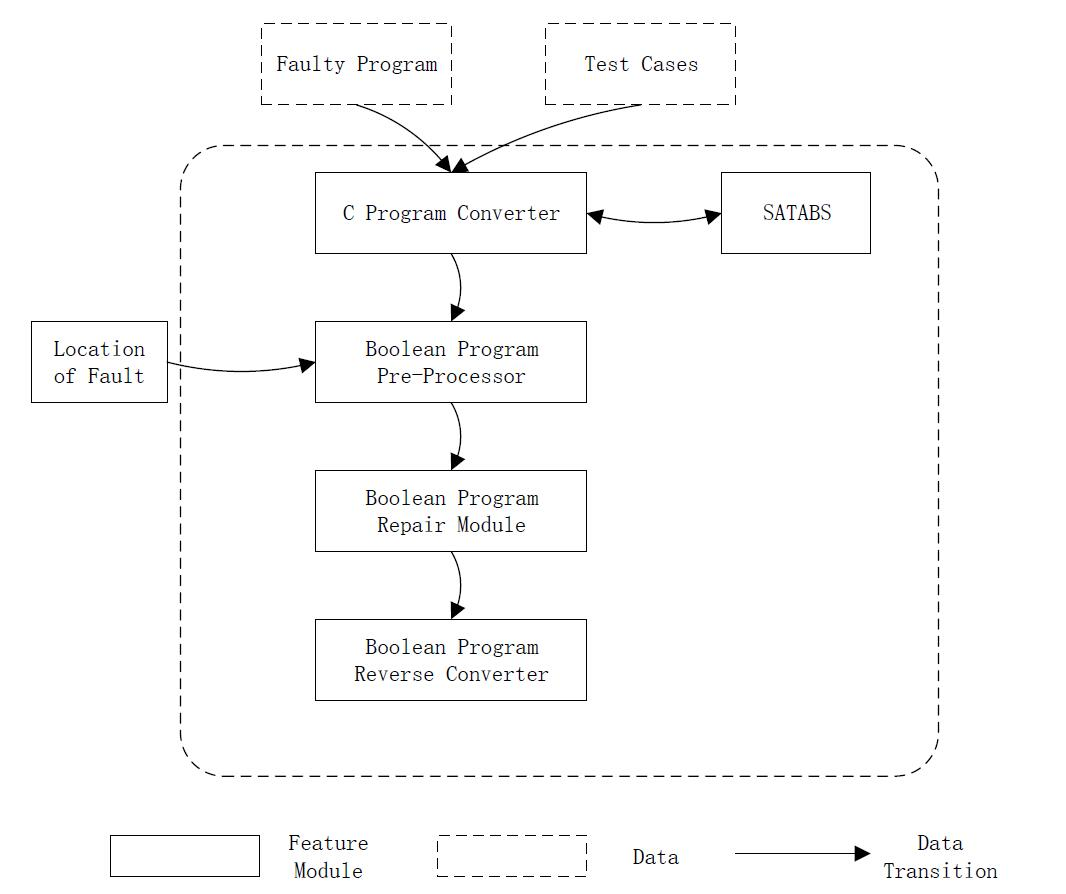
\includegraphics[width=4in,height=3.5in]{Fig4-1.jpg}
\caption{The Structure of the Tool}
\label{fig:SotT}
\end{figure}

\subsection{Modules of the Program Repair Tool}
We shall introduce you the details of these four components in this section.

\begin{itemize}
% C语言程序转换模块负责将C语言程序转换为布尔程序,同时对程序的变量和表达式进行谓词抽象。
\item \textbf{C program converter} is responsible for predicate abstraction and converting the given $C$ program to boolean program.
% 本模块主要调用了基于可满足性的程序抽象工具SATABS[2]来对原C语言程序进行转换。SATABS能处理C语言程序的赋值语句、控制流语句和函数调用语句等的转换,可以完成C语言程序到布尔程序的初步转换过程。
We use SATABS\cite{SATABS} to implement this module, which is capable of converting the assignment statements, control flow statements and invocation statements in $C$ program to the corresponding boolean program statements.
By doing so, this module achieves the basic conversion from $C$ program to boolean program.

\begin{itemize}
\item[-] \textbf{Input}: a faulty C program with given test cases and expected output.
\item[-] \textbf{Output}: the corresponding boolean program.
\end{itemize}

% 布尔程序预处理模块在一定程度上对C语言程序转换模块的完善。该模块对SATABS转换得出的布尔程序进行进一步的处理,
\item \textbf{Boolean program pre-processor} refines the converted boolean program to some extent. This module is capable of doing some further process on the converted boolean program,
% 去除文件中的无用信息,同时将布尔变量和其所代表的谓词以及C语言程序与布尔程序对应的位置关系提取出来。
including removing useless information, extracting the relations of boolean variables and predicates and the mappings from boolean statements to the original $C$ statements.
% 我们还在这里输入了原C语言程序出错语句的位置,使后续修复模块能够针对错误的位置进行修复。
We also input the location of the faulty $C$ statement in this process, leaving the information for further process in the following repair module.
% 本模块主要根据布尔程序的语法语义以及SATABS中C语言程序到布尔程序的转换规则对上一模块输出的文件进行分析和处理。
In summary, this module is responsible for analyzing and processing the boolean program given by last module based on the syntax and semantic of boolean programs and general conversion patterns of SATABS.

\begin{itemize}
\item[-] \textbf{Input}: a converted boolean program given by SATABS and the line number of the faulty $C$ statement in the original $C$ source file.
\item[-] \textbf{Output}: the refined boolean program and other useful related information.
\end{itemize}

% 布尔程序修复模块:对已知错误位置的布尔程序构建错误路径并计算得出正确的布尔修复。
\item \textbf{Boolean program repair module} constructs and collects all bad routes for the given boolean program and produces the appropriate boolean repair.
% 本模块可以细分为错误路径构建和修复求解两部分。
This module is actually made up of two parts: constructing bad routes and producing boolean repair.
% 错误路径构建主要是在已知错误位置的情况下,将错误语句用未知修复函数替代,并构造出所有的错误路径(见3.1.2节)。
As the location of the faulty statement is given, bad routes can be constructed by replacing the faulty statement with an unknown repairing function (\lstinline|*rep|) and listing all possible routes that lead to a wrong states (see section \ref{section:CollectingBadRoutes}).
% 修复求解则是在构建完错误路径后根据错误路径计算出修复函数的实现,即布尔修复(见3.1.3节)。
Further, the correct boolean repair will be calculated based on the set of all bad routes by taking the negation of their respective implementations (see section \ref{section:ProducingRepairingStatement}).

\begin{itemize}
\item[-] \textbf{Input}: the refined boolean program and related information.
\item[-] \textbf{Output}: boolean repair
\end{itemize}

\item \textbf{Boolean program reverse converter} converts the repaired boolean program back to $C$ language and finishes the repairing. First it will replace the boolean variables with their respective predicates
and determine the satisfiability of the converted repairing statement based on the SMT reduction described in section \ref{section:TheSatisfiabilityOfTheRepairingStatement}.
After this, several simplification rules will be applied on the converted repairing statement (section \ref{section:BooleanRepairSimplification}) to give out an effective and intuitive $C$ repairing statement.

\begin{itemize}
\item[-] \textbf{Input}: the boolean repair and the mappings produced by boolean program pre-processor.
\item[-] \textbf{Output}: the repaired $C$ program.
\end{itemize}

\end{itemize}

\subsection{Boolean Program Repair Module}
% 我们首先需要利用布尔程序修复模块找到布尔程序的正确修复。该模块又可以细分为错误路径构建和修复求解两部分。
First, boolean program repair module will be used to calculate the appropriate boolean repair. This module can be considered as two parts: constructing bad routes and calculating boolean repair.
% 在对布尔程序进行修复的时候,我们通过引入多个测试案例来确保修复结果的准确性。
Also, we improve the accuracy of this module by introducing more test cases.

% 对于一个给定的错误程序,我们需要构建出它所有可能到达错误终止状态的路径。
For a given faulty program, we need to constructs all possible routes that lead to wrong states.
% 本文以测试用例作为判断程序正确性的标准,通过assert语句来给出程序需要满足的规范,也即测试用例对应的正确输出结果。
We use test cases as the standard of a correct program in this paper, and define the specification a program should satisfy by \lstinline|assert| statements, meaning the expected output of test cases.
% 为错误程序构建错误路径时,我们会将错误语句所在的位置作为参数传入,将对应位置的语句替换为未知的修复函数,再将所有可能到达的错误状态的路径记录下来。
During the process of constructing bad routes, the location of the faulty statement will be passed as a parameter, and the faulty statement will be replaced by an unknown repairing function.
At this point, all possible bad routes will be constructed and recorded.

% 在求出了给定测试用例的所有错误路径之后,我们将对错误路径的并集取反来得到一条正确的执行路径,再进而计算该路径的具体实现。
After collecting all bad routes constructed by the given test cases, we negate the set of bad routes to produce the correct route, and further calculate the concrete implementation of this route.

\subsubsection{Multiple Test Cases Repair}
\label{section:MultipleTestCasesRepair}
% 为了确保修复结果的正确性,我们决定为一个错误程序引入多个不同的测试用例进行多次错误路径构建,从而使得到的错误路径能够完全覆盖。
More test cases means more bad routes can be constructed. In this sense, one can improve the coverage of bad routes by introducing more test cases, and by which improve the accuracy of the repairing.

% 3.1.2节中描述的代码修复方法能够根据给出的输入和正确的输出找出所有可能到达错误终止状态的错误路径。
The program repair method described in section \ref{section:CollectingBadRoutes} can find out all bad routes that lead to wrong states by given input and expected output.
% 当只给出一个测试用例时,程序的初始状态是确定的,因此在构建错误路径时所能得到的错误路径也是确定的。
For one single test case, the initial state of the program is determined, hance the bad routes can be constructed is determined.
% 不同的测试用例往往会有不同的初始状态,而在构建错误路径时,不同的初始状态到达错误状态的错误路径也是不相同的。
Different test cases can have different initial states, and different routes can be constructed to the same wrong state.
% 因此,在修复的过程中只引入一个测试用例来进行修复是不完备的。
Considering this, introducing only one test case when repairing is not completed.

% 我们针对同一个错误程序引入多个不同的测试用例,得到多个不同版本的C语言程序文件,
For one faulty program, different test cases can be introduced to generate $C$ source files of different versions.
% 再分别对它们进行错误路径构建和收集,最终再对这些结果进行分析,得出正确的修复结果。
We can still construct bad routes for each of them, and produce a more accurate repairing statement by collecting all these bad routes.
% 尽管不同版本的C语言程序转换为布尔程序后,布尔变量所代表的的谓词可能会有所不同,
$C$ source files of different versions can have different predicates and boolean variables,
% 但在找到错误路径后我们可以先对不同错误路径中的布尔变量进行合并,即对代表相同谓词的布尔变量统一命名。
but we can sum up the boolean variables in different bad routes, meaning unifying the names of boolean variables which stand for the same predicate.

\begin{theorem}
% 设引入一个测试用例对程序构建得到的错误路径集合为...,在此基础上增加测试用例对程序构建得到的错误路径集合为...,则有...。
Assume we have a set of bad routes $FP_{a}$ constructed by a test case $a$. If a new set of bad routes $FP_{b}$ can be constructed by introducing a new test case $b$,
we have $FP_{a} \subseteq FP_{b}$.
\end{theorem}

% 加入定义和定理引用
As defined in definition 3.6, the correct implementation of \lstinline|*rep| is calculated by negating the set of bad routes. If more test cases are introduces, based on theorem 4.1,
the coverage of bad routes constructed will be improved, meaning more wrong implementations of \lstinline|*rep| can be found. By doing so, we can improve the accuracy of the boolean repair.

\subsubsection{Pseudo Code}
% TO DO 插入图片并添加图片引用
% The detailed flow chart of boolean program repair module is shown in Figure 4-3, we will give out the basic implementation of this module in pseudo code in this section.

% 在对布尔程序修复构建错误路径的过程中,最重要的是模拟函数的运行过程直到终结状态通过assert语句确定该运行路径是否是错误路径
The key of constructing bad routes is to simulate the execution of the simulated function until a termination state is reached, and determine if this route is a bad route by \lstinline|assert| statement and the current evaluation.
% 模拟函数运行构建错误路径的算法基本思想是采用深度优先搜索,在进入函数时找到所有可能到达的状态,再对所有可能到达的状态进行下一步模拟进行。
All possible routes starting from a given state can be considered as a tree, while the given state being the root of the tree. The algorithm collects all possible bad routes by iterating the whole tree in a depth-first manner,
guaranteeing every state will be iterated, hence every possible route.

The pseudo code of this algorithm is shown as follows:

\begin{algorithm}
\caption{Function simulating algorithm}
\begin{algorithmic}[1]

\STATE $\textit{func} \gets \text{the function being simulated}$
\STATE $\textit{loc} \gets \text{the location of the statement being simulated}$
\STATE $\textit{eva} \gets \text{the current evaluation}$
\STATE $\textit{route} \gets \text{the current route}$
\STATE $\textit{states} \gets \text{list of all possible next states}$
\STATE $\textit{bad\_routes} \gets \text{the list of all recorded bad routes}$
\STATE

\IF {$loc == 0$}
  \IF {$\textit{loc}$ has already been simulated for $\textit{func}$}
    \RETURN existed result
  \ENDIF
\ENDIF

\STATE
\STATE push the current state to \textit{route}

\STATE
\STATE $\textit{st} \gets \textit{func}[\textit{loc}]$

\IF {$\textit{st}$ is an assignment statement}
  \IF {$\textit{st}$ is not the unknown repairing statement}
    \STATE push next state to \textit{states}
  \ELSE
    \STATE push every possible next state to \textit{states}
  \ENDIF
\ELSIF {$\textit{st}$ is an `if` statement}
  \IF {$\textit{st}$ is not the unknown repairing statement}
    \STATE push next state to \textit{states}
  \ELSE
    \STATE push every possible next state to \textit{states}
  \ENDIF
\ELSIF {$\textit{st}$ is a `goto` statement}
  \STATE push the destination state to \textit{states}
\ELSIF {$\textit{st}$ is an invocation statement}
  \STATE push every possible next state to \textit{states}
\ELSIF {$\textit{st}$ is an `assert` statement}
  \IF {$\textit{st}$ is the unknown repairing statement}
    \IF {$!check\_assert(st, eva)$}
      \STATE add \textit{route} to \textit{bad\_route}
      \RETURN the result
    \ENDIF
  \ENDIF
\ELSE
  \IF {\textit{loc} \text{is at the end of} \textit{func}}
    \RETURN the result of \textit{func}
  \ENDIF
\ENDIF

\STATE
\FORALL {state \textit{s} in \textit{states}}
  \STATE simulate \textit{s} in \textit{func}
\ENDFOR

\STATE
\IF {$loc == 0$}
  \STATE cache the result of \textit{func}
\ENDIF

\STATE
\STATE pop the current state from \textit{route}
\end{algorithmic}
\end{algorithm}

% 至此,我们已经找到了这个程序的所有错误路径,现在需要从这些错误路径中计算得到修复
So far, we collect all bad routes of a boolean program by applying the algorithm above, the next thing we need to do is to produce an appropriate boolean repair from these bad routes.
% 在3.1节中,已经证明,一个正确的修复应该不通过任意一个错误状态
In section \ref{section:BooleanProgramRepair}, we have proved that a correct boolean repair should be lead to any wrong states.
% 在每个错误路径中各取一个路径取非,再把所得路径取合取,就得到了一条正确路径
For every bad route we negate it, and conjunct all these resulting routes, and the result will be a correct path.

\begin{algorithm}
\caption{Calculates boolean repair}
\begin{algorithmic}[1]
\STATE $\textit{good\_route} \gets \text{a empty list}$
\STATE

\FORALL {\textit{route} in \textit{bad\_route}}
  \STATE negates any element of \textit{route} then put it into \textit{good\_route}
\ENDFOR

\STATE
\RETURN \textit{good\_route}

\end{algorithmic}
\end{algorithm}

% 现在计算得到了good_route,它展示了正确的*rep函数在不同的变量下的返回值,现在需要把*rep用布尔表达式表示出来。
For now, we have \lstinline|good\_route|, which stands for the correct implementation of $*rep$, represented as pairs of input and expected output of $*rep$. The last thing to do is to convert it to a readable boolean expression.
% 例如 *rep(00)=1 , *rep(01)=0 ,如果直接地表示这个布尔表达式,则应该为...
For example, we have something like $*rep(00) = 1$, $*rep(01) = 0$. Apparently, the boolean expression can be $\cap{p_{0}p_{1}} || \cap{\cap{p_{0}}p_{1}}$,
% 显然当变量多时,这种表示方式既不直观,也不方便后面的化简计算,因此我们需要更好的方式表示它。
but such representation can be complicated when the number of variables goes up, which is also difficult for further simplification.
Hence, a better representation is needed.

% 这里的实现采用了二分决策图的方法
In this case, the concept of Binary decision diagram\cite{BDD} can be introduced.
% 二分决策图是用来表示布尔函数的压缩型数据结构
The binary decision diagram (BDD) is a data structure for representing Boolean functions, which can also be considered as a compressed representation of sets or relations\cite{TfEFVUBDD,FtOVOfBDD}.
% 布尔函数可以表示为一个有根定向无环图,其中包括了决策节点和两个终端节点表示真和假,每个决策节点都被标记为一个布尔变量。一条从根节点
A Boolean function can be represented as a rooted, directed, acyclic graph, which consists of several decision nodes and terminal nodes. There are two types of terminal nodes called 0-terminal and 1-terminal.
Each decision node $N$ is labeled by boolean variable $V_{N}$ and two child nodes, representing setting the variable to $true$ or $false$.
% 一条从根节点到真值终端的路径表示该路径所代表的的变量赋值使得该布尔函数为真。
A path from the root node to a 1-terminal node means the values of variables represented by this path makes the expression to be $true$.
% 二分决策图能够消除布尔变量赋值中的冗余信息,使得其比普通的真值表表示要小很多,能够极大地压缩搜索空间
BDD can be used to eliminate duplicate information from a given boolean expression, as equivalent expressions will always produce a same BDD. Also, the representation of BDD is generally smaller than truth table,
by which the search space can be greatly reduced.

% 除了使用BDD,也可以把上面的布尔表达式展开成析取范式,并适用3.4节所证明的方法进行逻辑化简
Except for BDD, logic simplification rules described in section \ref{section:BooleanRepairSimplification} can also be applied after converting the given expression into DNF.

\subsection{Boolean Repair Reverse Converter}
% 通过布尔程序修复,我们得到了针对布尔程序的布尔修复
By applying the algorithm described in the former section, we have the boolean repair for boolean program.
% 布尔修复是由布尔变量组成的布尔表达式
Boolean repair is a boolean expression consisted of boolean variables.
% 为了得到C语言程序的修复结果,我们还需要将其转换为C语言表达式,并判断转换后的结果是否是正确且有效的。
To repair the original $C$ program, we still need to convert it to a $C$ statement and determine if the converted repairing statement is correct and effective.

% TO DO 插图,加入图片引用
% The detailed flow chart of reverse converter is shown in figure 4-4.

% 在布尔修复逆向转换模块的实现中,首先需要将布尔修复语句转换为谓词公式,在对公式的子句间和子句内进行化简
During the conversion, the first thing to do is to convert the boolean repair to its respective predicate formula.

\begin{algorithm}
\caption{Conversion of repairing clauses}
\begin{algorithmic}[1]

\STATE $\textit{clause\_str} \gets \text{the conjunctive clause to be converted}$
\STATE $\textit{vars\_map} \gets \text{mappings from boolean variables to predicates}$
\STATE $\textit{predicates} \gets \text{the list of converted predicates}$
\STATE

\STATE $\textit{vars\_str} \gets \text{split}(\textit{clause\_str}, \text{"\&"})$
\FORALL {\textit{var\_str} in \textit{vars\_str}}
  \STATE $\textit{isNeg} \gets \text{if the current variable is a negation}$
  \IF {\textit{var\_str}[0] == \textit{'!'}}
    \STATE $\textit{isNeg} \gets true$
    \STATE $\textit{var\_str} \gets \textit{var\_str}.\text{substr}(1)$
  \ELSE
    \STATE $\textit{isNeg} \gets false$
  \ENDIF
  \STATE
  \STATE $\textit{predicate} \gets \textit{vars\_map}.map(\textit{var\_str})$
  \IF {\textit{isNeg}}
    \STATE $\textit{predicate} \gets \textit{predicate}.\text{negate}()$
  \ENDIF
  \STATE \textit{predicates}.push(\textit{predicate})
\ENDFOR
\STATE
\RETURN \textit{predicates}

\end{algorithmic}
\end{algorithm}

\begin{algorithm}
\caption{Conversion of repairing expression}
\begin{algorithmic}[1]

\STATE $\textit{expr\_str} \gets \text{the disjunctive expression to be converted}$
\STATE $\textit{clauses} \gets \text{the list of converted clauses}$
\STATE

\STATE $\textit{clauses\_str} \gets \text{split}(\textit{expr\_str}, "\mid")$

\FORALL {\textit{clause\_str} in \textit{clauses\_str}}
  \STATE $\textit{clause} \gets \text{clause\_conversion}(\textit{clause\_str})$
  \IF {\textit{clause} is always \textit{true}}
    \RETURN always \textit{true}
  \ENDIF
  \STATE \textit{clauses}.push(\textit{clause})
\ENDFOR

\end{algorithmic}
\end{algorithm}

As the repairing statement generated by the tool will always be in DNF, simplification can be applied to produce a more readable statement.
Several effective simplification rules are described in section \ref{section:BooleanRepairSimplification}, while applying BDD for simplification is also acceptable.

\subsection{Complexities of Algorithms}
% 前文给出了布尔程序修复逆向转换工具的具体实现及算法,该工具可以看作一个整体的完善的修复系统。我们将在这里给出工具每个模块实现算法的时间复杂度的分析。
In the former sections, we described the basic implementation of the program repair tool. In this section, the time complexity of different modules will be analyzed.

% C程序转换模块调用了外部的SATABS程序来将C程序转换为布尔程序,因此这部分的算法复杂度不作考虑。
The $C$ program converter is implemented by using SATABS to convert a $C$ program to boolean program, hence the complexity of this module will not be considered.

% 布尔程序预处理模块算法的时间复杂度是常数级别的
The algorithm used to implement boolean program pre-processor is constant time.
% 该模块提取除了布尔程序的变量个数以及C程序语句和布尔程序语句的映射关系
This module is responsible for extracting the information of boolean variables and the mappings from $C$ statements to boolean statements.
% 具体实现时利用了SATABS对C程序转换为布尔程序过程中产生的信息,只需要对C程序和布尔程序各查找常数次
Such intermediate information will be generated when SATABS is converting the $C$ program, constant number of searches on both source files is all we need.
% 设转换前的C程序行数为LoC,转换后的布尔程序的行数为LoBP,则这部分算法的复杂度为...
If we have to consider the length of source files, let's assume the number of lines in the original $C$ program is $LoC$ and the converted boolean program is $LoBP$,
then the complexity of this algorithm should be $O(LoC + LoBP)$.

% 布尔程序修复模块部分的算法复杂度是整个工具的瓶颈
The boolean program repair module is actually the bottleneck of the whole system.
% 设布尔程序的变量个数为.., 则布尔程序运行过程中,变量的赋值空间为...,因此总的可能的运行路径数为...在程序运行过程中产生的不同的状态数为...
Assume the number of boolean variables is $V$, then the number of evaluations could be $X = O(2^{V})$, which means the number of possible routes is $O(2^{X})$,
and the number of distinct states is $O(LoBP * X)$.
In this sense, the number of routes grows exponentially as the number of boolean variables grows, which also grows exponentially as the number of variables in the original $C$ program grows. It would appear to be the major bottleneck of the whole system. The complexity of this module is $O(LoBP * X + 2^{X})$.

% 在整个布尔程序逆向转换工具中,布尔程序修复算法是整个系统的瓶颈所在,因此需要对其进行优化。
As the bottleneck of the whole system, optimization can be applied on this module.
% 在本文的实现中,采用了减少模拟运行过程中需要考虑的变量数来进行优化,即减少V的大小
In our implementation, we use different ways to reduce the number of variables need to be considered during the simulation, meaning reducing $V$.
% 由于 X = 2^V,V的减少会对算法的复杂度进行极大地优化
As $X = 2^{V}$, no doubt the reduction on $V$ can greatly facilitate the performance of the algorithm.
% 这种优化方法是可行且正确的,因为在每一步的运算过程中,大部分变量都为临时变量或与当前运算不相关的变量,
Such optimization is actually effective, as for each statement, most accessible variables are of temporary use or irrelevant to the simulating statement.
% 因此可以只将当前的非临时且与运算有关的变量提取出来,只考虑这些变量在路径中的状态变迁。
In this case, we only consider the state transitions of those variables which is not temporary and is relevant to the current statement during the simulation.
% 这将使得布尔程序修复部分的运行时间大幅减少并在可接受范围内
By doing so, the time cost needed for boolean program repair is greatly reduced and become more acceptable.

% 在布尔修复逆向转换模块,最关键的工作是将一个布尔程序语句转换成C程序语句并根据语义进行化简。
Boolean repair reverse converter is responsible for converting boolean statement back to respective $C$ statement and apply simplification based on its semantic.
% 在整个转换及化简的过程中,修复表达式始终保持为析取范式。
Note that the repairing expression will maintain to be in DNF in the whole process.
% 设析取范式的修复子式个数为N,每个修复子式中最大的谓词个数为M。
Assume the number of clauses in the DNF expression is $N$, and the maximum number of predicates in each clause is $M$.
% 对一个修复子式执行子句内化简时,将谓词按照它们的语义进行排序,并合并了语义可化简的谓词。
During the process of inner-clause simplification, predicates will be sorted based on their semantics, and those predicates with similar semantics will be combined as one.
% 谓词的排序可以采用快速排序,算法的复杂度为O(MlogM),而排序后可合并的谓词只会相邻出现,因此合并的算法复杂度为O(M)。
The sort of predicates can be implemented by quick sort, whose complexity is $O(M\log{M})$. After the predicates are in order, those predicates with combinable semantics will only appear consecutively,
so the complexity of finding combinable predicates is $O(M)$.
% 由此,对所有修复子式执行子句内化简的算法复杂度为O(NMlogM)。
In this sense, the complexity of inner-clause simplification for all clauses is $O(NM\log{M})$.
% 执行子句间化简时,需要枚举两个修复子式,并检查两个修复子式中每个谓词的含义是相同还是相反,因此算法的时间复杂度为O(N^2M^2)
Each pair of clauses will checked for whether their predicates have same or exactly opposite meanings in the process of inter-clause simplification, hence the complexity is $O(N^{2}M^{M})$.
% 执行子句外化简时,需要检查每个子句的可满足性,而检查子句的可满足性属于SMT问题。
As for outer-clause simplification, the satisfiability of each clause will be examined, which can be reduced to SMT problem.
% SMT问题是个NP完全问题,不存在多项式时间算法,因此最坏情况下的时间复杂度为O(2^M)。
SMT program is an NP-complete problem, which can be verified in polynomial time, so the complexity of outer-clause simplification will be $O(2^{M})$ in the worst case.
% 由于先执行了子句内化简,子句中的谓词数量减少,能有效地降低时间复杂度。
But outer-clause simplification actually preforms after inner-clause simplification, which can reduce the number of predicates in clauses, hence reduce the time cost needed for outer-clause simplification.
% 因此,布尔修复逆向转换的总体复杂度为...
In summary, the time complexity of boolean repair reverse conversion is $O(NM\log{M} + N2^{M} + N^{2}M^{2})$.

\newpage
\section{Experiment}
\label{section:Experiment}
% 为了验证本文方法及工具的可行性与正确性,本章给出了对布尔程序逆向转换修复的测试实验。
To verify the effectiveness and correctness of the methods and tool described in former sections, detailed experimental results and analysis will be given in this following section.
% 本章实验通过对现有的标准程序进行修复和转换,从修复结果的准确率和修复的效率等方面对布尔程序逆向转换工具进行评价
In the experiment, the program repair tool will be used to repair some programs and evaluated based on its accuracy and efficiency.

% 在本章的实验中,主要针对工具能够修复的赋值错误和控制条件语句错误进行了修复及转换测试
The experiment mainly tested the tool on its ability to convert and repair assignment statements and conditional control flow statements (\lstinline|if|).
% 其中选取了在程序诊断中比较常用到的西门子套件中的TCAS程序以及一些针对TCAS未能覆盖的循环语句条件错误的测试程序。
To be more specific, Several test cases of TCAS program from Siemens Suite, which has been used as a benchmark to evaluate the effectiveness of many testing techniques, are used in this experiment. More customized programs are added to the test cases to test the tool's ability of repairing boolean expression faults in loop statements, which Siemens' TCAS fails to cover.

\subsection{TCAS of Siemens Suite}
\subsubsection{Introduction}
% TCAS程序是程序诊断的基准测试用例集西门子套件中的其中一个程序,
The TCAS program used in the experiment comes from Siemens Suite, which has been used by other recent works on fault localization\cite{EotEoDaCBTAC,ESoaRTST}.
% 该程序的主要功能是模拟飞机调度中产生冲突的情况及给出了防止飞机相撞的办法。[51]
TCAS, or traffic collision avoidance system, is an aircraft collision avoidance system designed to reduce the incidence of mid-air collisions between aircraft\cite{TCAS}.
% TCAS有正确版本的程序以及41个不同错误版本的错误程序,此外,在TCAS的基准套件中还给出了1608个不同的测试用例输入。
Siemens Suite provides a correct TCAS program, along with 41 different faulty versions. Additionally, 1608 different test cases are provided in Siemens Suite.
% 程序长度为173行,包含25个全局变量,除main函数外还有其他8个函数,因此程序中有函数调用。
The program has 173 lines of statements, including 25 global variables and 8 functions except for \lstinline|main| function.
% 在给出的41个不同错误版本中,V10、V11、V15、V31、V32、V33、V40的版本中包含多个错误,不在本文的修复考虑行列,因此不做统计。
Among the 41 given faulty versions, $V10$, $V11$, $V11$, $V15$, $V31$, $V31$, $V32$, $V33$, $V40$ contain multiple faults in one file, which is not supported by the tool, hence they will not be considered in the experiment.
% 表5-1给出对了TCAS程序的其余34个错误版本的错误类型统计,其中修复错误归类为赋值语句右部错误以及控制条件语句错误的版本为本文能够修复的错误。
The statistics of the rest 34 versions is listed in table \ref{table:SoTCASTC}, in which assignment statement fault and conditional control flow statement fault are supported by the tool.

\begin{table}
\small
\center
\caption{Statistics of TCAS Test Cases}
\label{table:SoTCASTC}
\begin{tabular}{lll}
\hline
Version                                 & Fault Type                  & Detailed Fault Type         \\
\hline
$5$,$21$,$22$,$23$,$24$,$27$,$41$       & Assignment Statement Fault  & Logical Error in Assignment \\
$1$,$3$,$4$,$6$,$9$,$12$,$20$,$25$,$39$ & Assignment Statement Fault  & Wrong Operator              \\
$13$,$14$,$16$,$17$,$18$,$19$,$36$,$38$ & Declaration Error           & Declaration Error           \\
$2$,$28$,$29$,$30$,$35$,$37$            & Assignment Statement Fault  & Wrong `return` Statement    \\
$7$,$8$                                 & Assignment Statement Fault  & Initialization Error        \\
$34$                                    & Conditional Statement Fault & Wrong Condition Expression  \\
\hline
\end{tabular}
\end{table}

\subsubsection{Preprocess on Test Cases}
% TCAS程序在运行的时候需要读取参数作为输入,但是本修复工具在C程序转换为布尔程序的过程中,C程序已经包含了测试用例,即程序的输入和输出已经加进了C程序之后才将其转换为布尔程序。
To execute the TCAS program, designated input is needed, but the repair tool we design assumes the given $C$ program already includes test case.
% 因此针对每个错误版本的C程序,首先将选定的一个或多个测试用例直接赋给相关需要读入参数的变量,并且将预期输出结果以”assert(output ==  expected)"的形式加在main函数返回语句之前。
In this case, for each faulty version, one or more test cases will be selected to assign to the respective input variables, while new \lstinline|assert| statement will be added just before the end of \lstinline|main| function
to examine the program's output.
% 程序在加入测试用例的输入和预期输出后则表示给出了程序的行为规范,assert语句规定了程序的正确终止状态,因此如果在模拟函数运行的过程中路径到达的状态不满足当前的assert语句,则表示到达的是错误终止状态,即该路径是错误路径。
By doing so, the given input and expected output of the test cases give out the specification of the program's behavior.

% 在对TCAS的修复实验中,为了验证前文提到的多个测试用例修复方法还进行了当程序只加入一个测试用例输入以及加入多个测试用例输入时的结果对比。
In the TCAS repairing experiment, we introduced different numbers of test cases to one faulty version, hoping to prove the effectiveness of the multi-test-case repair method we described in section \ref{section:MultipleTestCasesRepair}.

\subsubsection{Experimental Results}
% 针对表5-1中可以被修复的26个程序版本进行了实验,对于这些版本的错误, 使用多个测例进行修复并转换的方法均能找到程序的修复。
We experimented on the 26 faulty versions listed in table \ref{table:SoTCASTC} whose faults are supported by the tool. For the faults of these versions, the repairing method which uses multiple test cases managed to locate all of them.

% 表5-2列举了其中10个版本的程序的测试实验结果。
% TODO 加入表格引用
The results of 10 of them are listed in table \ref{table:RoTCASTC}. Meanings of columns in table \ref{table:RoTCASTC} are listed below:

\begin{enumerate}
\item {\it Version}   : the version number.
\item $V$             : the number of global and relevant boolean variables.
\item $LoBP_{1}$      : the length of converted boolean program when only one test case is introduced.
\item $Time_{1}$($s$) : the time in seconds used to repair the given boolean program when only one test case is introduced.
\item $Result_{1}$    : the percentage of passed tests among the given 1608 tests when only one test case is introduced.
\item $LoBP_{2}$      : the length of converted boolean program when multiple test cases are introduced.
\item $Time_{2}$($s$) : the time in seconds used to repair the given boolean program when multiple test cases are introduced.
\item $Result_{2}$    : the number of test cases which cover bad routes effectively and the number of test cases we use.
\end{enumerate}

We shall give you a detailed insight into one of them. Takes $V1$ as an example, we used 6 test cases to find out a correct repair statement, which was $*rep=(b4)|(b3)|(b2)|(!b1)|(b0)$ with respective predicates of each variable listed below:

\begin{itemize}
\item[-] $\text{b0} : \textit{Down\_Separation} - \textit{Positive\_RA\_Alt\_Thresh}[\textit{Alt\_Layer\_Value}] == 0$
\item[-] $\text{b1} : \textit{Down\_Separation} - \textit{Positive\_RA\_Alt\_Thresh}[\textit{Alt\_Layer\_Value}] <= 0$
\item[-] $\text{b2} : \textit{Other\_Tracked\_Alt} - \textit{Own\_Tracked\_Alt} <= 0$
\item[-] $\text{b3} : \textit{Down\_Separation} - \textit{Positive\_RA\_Alt\_Thresh}[\textit{Alt\_Layer\_Value}] >= 0$
\item[-] $\text{b4} : \textit{Down\_Separation} - \textit{Up\_Separation} >= 100$
\end{itemize}

Judging from the experimental result, $*rep$ is satisfiable. After applying the simplification rules we described in former section, we have a converted $C$ repair statement \lstinline|Down_Separation - Positive_RA_Alt_Thresh[Alt_Layer_Value] < 0| \lstinline| && | \lstinline|Down_Separation - Up_Separation < 100| \lstinline| && | \lstinline|Other_Tracked_Alt - Own_Tracked_Alt > 0|. After replacing the faulty statement with the above statement, the repaired program passed all test cases.

\begin{table}
\small
\center
\caption{Results of TCAS Test Cases}
\label{table:RoTCASTC}
\begin{tabular}{|c|c|c|c|c|c|c|c|}
\hline
Version & $V$     & $LoBP_{1}$ & $Time_{1}$($s$) & $Result_{1}$ &$LoBP_{2}$ & $Time_{2}$($s$) & $Result_{2}$ \\
\hline
$1$     & $6/22$  & $806$      & $66.6$          & $95.0\%$     & $714$     & $474.1$         & $6/10$       \\
\hline
$3$     & $2/15$  & $894$      & $101.0$         & $97.5\%$     & $749$     & $717.4$         & $3/10$       \\
\hline
$4$	    & $10/16$ & $697$      & $132.9$         & $100\%$      & $591$     & $250.7$         & $6/10$       \\
\hline
$5$	    & $4/18$  & $803$      & $50.2$          & $100\%$      & $506$     & $339.5$         & $5/10$       \\
\hline
$6$	    & $5/19$  & $717$      & $43.3$          & $99.8\%$     & $514$     & $220.3$         & $2/10$       \\
\hline
$9$	    & $7/24$  & $928$      & $96.1$          & $93.5\%$     & $815$     & $751.2$         & $6/10$       \\
\hline
$12$    & $4/17$  & $816$      & $358.3$         & $99.9\%$     & $852$     & $920.6$         & $4/10$       \\
\hline
$26$    & $4/18$  & $803$      & $51.3$          & $99.9\%$     & $52$      & $526.7$         & $6/10$       \\
\hline
$27$    & $4/18$  & $803$      & $50.8$          & $99.9\%$     & $520$     & $432.7$         & $5/10$       \\
\hline
$34$    & $3/17$  & $856$      & $105.3$         & $83.2\%$     & $835$     & $665.6$         & $4/10$       \\
\hline
\end{tabular}
\end{table}

\subsection{Cases of Loop Fault}
\subsubsection{Introduction of Test Cases}
% TCAS程序中涉及到控制条件语句错误的版本只有函数调用、选择控制和赋值等语句,而没有循环语句结构,
Loop statement fault is the kind of fault which the TCAS from Siemens Suite fails to cover.
% 因此为了验证本文工具的修复功能的全面性,在测试的过程中又增加了两组程序,这两组程序分别包含了while循环和for循环语句结构,
In this case, two groups of customized programs are added to the experiment. Both groups implement the algorithm of finding the maximum value of a given array.
% 程序实现的功能是查找给出数组中最大的数。
The difference is, one group is implemented by \lstinline|while| loop while the other is \lstinline|for| loop.

% 本实验中分别对每个程序给出了两个错误的版本(如图5-1所示),版本1的错误位置分别出现在while和for循环中的循环控制条件中,版本2的错误位置则出现在循环体内的if控制条件语句内。
Two faulty versions of both programs are respectively given in Figure \ref{fig:WaF}, in which fault 1 is located in the condition expression of loop statement, while fault 2 is located in the \lstinline|if| statement in the loop body.

\begin{figure}
\centering
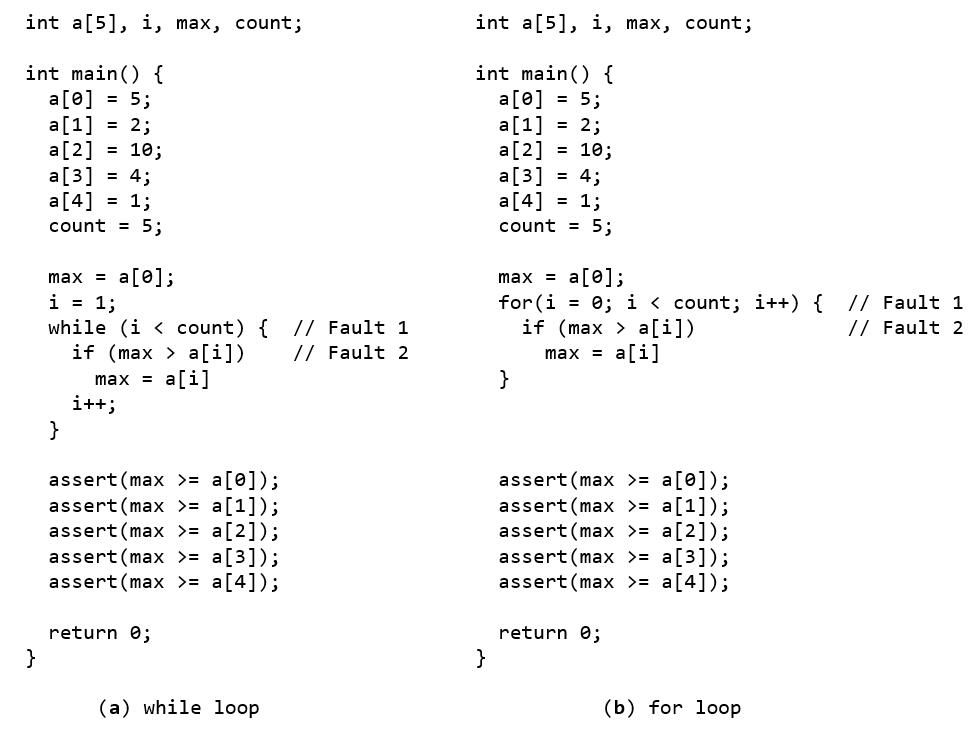
\includegraphics[width=5in]{img/Fig5-1.jpg}
\caption{While loop and for loop faulty programs}
\label{fig:WaF}
\end{figure}

\subsubsection{Experimental Results}
% 对while和for循环的两个错误版本中只需要采用一个测试用例便可以得到修复的结果
For loop statement fault, one test case is sufficient for finding the repairing statement.
The results are listed in table \ref{table:RoCTC}. Meanings of columns in table \ref{table:RoCTC} are listed below:

\begin{enumerate}
\item {\it Version}: the version number of the corresponding version.
\item $V$             : the number of global and relevant boolean variables.
\item $LoBP_{1}$      : the length of converted boolean program when five test cases are introduced.
\item $Time_{1}$($s$) : the time in seconds used to repair the given boolean program when five test cases are introduced.
\item $Result_{1}$    : the percentage of passed tests among the given 2000 tests when five test cases are introduced.
\item $LoBP_{2}$      : the average length of converted boolean program when multiple test cases are introduced.
\item $Time_{2}$($s$) : the time in seconds used to repair the given boolean program when multiple test cases are introduced.
\item $Result_{2}$    : the number of test cases which cover bad routes effectively and the total number of test cases we use.
\end{enumerate}

\begin{table}
\small
\center
\caption{Results of Customized Test Cases}
\label{table:RoCTC}
\begin{tabular}{|c|c|c|c|c|c|c|c|}
\hline
Version   & $V$     & $LoBP_{1}$ & $Time_{1}$($s$) & $Result_{1}$ &$LoBP_{2}$ & $Time_{2}$($s$) & $Result_{2}$ \\
\hline
$while_1$ & $4/40$  & $177$      & $0.38$          & $89.6\%$     & $177$     & $14.1$          & $10/100$     \\
\hline
$while_2$ & $5/40$  & $178$      & $0.31$          & $58.3\%$     & $178$     & $2.7$           & $2/100$      \\
\hline
$for_1$   & $4/40$  & $177$      & $0.26$          & $89.6\%$     & $177$     & $14$            & $10/100$     \\
\hline
$for_2$   & $5/40$  & $178$      & $0.30$          & $58.3\%$     & $178$     & $2.9$           & $2/100$      \\
\hline
\end{tabular}
\end{table}

% 从实验结果可以看出对于包含while和for循环结构的程序的循环控制条件语句错误以及if控制条件语句错误,本文所设计的布尔程序修复逆向转换工具也能对其进行修复,进一步验证了本文所设计工具的有效性。
Judging from the experimental results, the tool is capable of handling loop statement fault and conditional control flow statement fault, which also provides convincing evidence of the tool's effectiveness.

% 在附录一中将会给出本章实验的具体测试用例的错误语句、布尔程序修复语句以及转换后的修复结果语句。
% TODO 添加附录引用
In Appendix \ref{appendix:ExperimentalDataandResults}, the concrete test cases we used in the experiment and the respective boolean repairs and converted $C$ repairing statements will be listed respectively.

\subsection{Conclusions}
% 本章的实验结果数据表明本文的方法对于控制条件错误和赋值语句右部错误例如赋值逻辑错误、操作符错误、返回语句错误等程序里实际存在的错误能够给出实际有效且符合坃程序语法语义的修复结果。
Based on the experimental results listed in the former sections, one can say the tool is capable of producing an effective and intuitive repair statement for many kinds of faults, including assignment statement fault and conditional control flow statement fault, which generally exist in most faulty programs.

% Griesmayer[18]在2005年的工作自动找到布尔程序的修复结果之后需要通过程序员人工地将结果转换为布尔程序的结果,没有达到自动化的目的。
In 2005, Griesmayer managed to find the boolean repair automatically\cite{RoBPwaAtC}, but manual intervene is still needed to convert the boolean repair back to the original programming language. In this sense, Griesmayer's work failed to achieve complete automation for program repair.
% 实验结果表明本文的工作完成了程序修复的自动化过程,能够直接地找到坃程序的有效修复。
Judging from the experimental results, our tool is capable of completing the whole process of program repair automatically and producing an effective repair statement.

% Weimer[22]在2009年提出的利用遗传算法来进行程序修复的方法修复的是死循环和段错误以及堆栈溢出等错误类型,并没有实验结果显示能够修复具体的赋值逻辑错误和操作符错误等。
In 2009,  Forrest and Weimer for the first time apply evolutionary computation to repair a real-world software system\cite{AFPUGP}. Their repairing system was capable of repairing faults like
infinite loop and stack overflow, but there was no experimental result that proved their tool supports assignment fault or control flow fault.
% 本文能够修复的错误类型更多的是程序语句逻辑上的错误,与Weimer等人解决的问题领域有差别。
The fault model we discussed in this paper focuses on logical faults of program statements, which makes a difference from Weimer's study.

\newpage
\section{Summary}
% 在本文中,我们介绍了如何将C语言程序转换为布尔程序,通过收集布尔程序的错误路径得出正确的布尔修复,并介绍了该如何验证该布尔修复的可满足性
In this paper, we illustrated the basic conversion rules from $C$ program to boolean program,
and by collecting bad routes for the converted program, we managed to produce an appropriate boolean repair for a faulty program.
Examination of the satisfiability of the boolean repair is also introduced in the paper.
% 最终,通过对布尔修复进行化简,我们得到了正确有效且相对直观的C语言修复表达式。
At last, by simplifying the boolean repair, an effective and relatively intuitive $C$ repairing statement is generated.
% 我们还对实现的工具进行了大量的测试,证明了该方法对于TCAS测试集中的赋值语句错误和控制语句错误都能找到正确的修复结果。
A lot of tests are also performed on the program repair tool, proving that the method described in this paper is capable of repairing assignment statement faults and control flow statement faults of TCAS.

% 本文设计并实现的布尔程序修复工具,在功能上仍有改进的空间。
There are still more work to be done on the program repair tool.
% 在布尔程序修复模块,尽管能够找到正确的修复,但是修复的时间和空间复杂度较高,
For the boolean program repair module, though it is capable of finding a correct repairing statement, it comes with significantly high time complexity.
% 当布尔变量数增加时,复杂度会呈指数级增长,制约了修复的效率
The time cost will grow exponentially as the number of variables grows, which limits its availability for real-world programs.
% 因此下一步的工作中将对修复算法的搜索进行优化。
In this case, further work can be done on optimizing the search algorithm used in this module.
% 除此之外,本文所使用的错误模型只适用于单行语句的错误,这其中只包括了很少一部分简单错误。下一步工作也将继续扩展支持的错误类型,如死循环和程序的语句缺失错误等。
Besides, the fault model defined in this paper only supports those faults lying in one single statement, which include only a few kinds of faults.
Hence, supporting more kinds of faults, such as infinite loop and missing statements, can also be considered for further improvement.

\newpage
\bibliography{bpr}{}
\bibliographystyle{ieeetr}

\end{document}
